%%%%%%%%%%%%%%%%%%%%%%%%%%%%%%%%%%%%%%%%%
% Masters/Doctoral Thesis 
% LaTeX Template
% Version 2.5 (27/8/17)
%
% This template was downloaded from:
% http://www.LaTeXTemplates.com
%
% Version 2.x major modifications by:
% Vel (vel@latextemplates.com)
%
% This template is based on a template by:
% Steve Gunn (http://users.ecs.soton.ac.uk/srg/softwaretools/document/templates/)
% Sunil Patel (http://www.sunilpatel.co.uk/thesis-template/)
%
% Template license:
% CC BY-NC-SA 3.0 (http://creativecommons.org/licenses/by-nc-sa/3.0/)
%
%%%%%%%%%%%%%%%%%%%%%%%%%%%%%%%%%%%%%%%%%

%----------------------------------------------------------------------------------------
%	PACKAGES AND OTHER DOCUMENT CONFIGURATIONS
%----------------------------------------------------------------------------------------

\documentclass[
11pt, % The default document font size, options: 10pt, 11pt, 12pt
%oneside, % Two side (alternating margins) for binding by default, uncomment to switch to one side
english, % ngerman for German
onehalfspacing, % Single line spacing, alternatives: onehalfspacing or doublespacing
%draft, % Uncomment to enable draft mode (no pictures, no links, overfull hboxes indicated)
%nolistspacing, % If the document is onehalfspacing or doublespacing, uncomment this to set spacing in lists to single
%liststotoc, % Uncomment to add the list of figures/tables/etc to the table of contents
%toctotoc, % Uncomment to add the main table of contents to the table of contents
%parskip, % Uncomment to add space between paragraphs
%nohyperref, % Uncomment to not load the hyperref package
headsepline, % Uncomment to get a line under the header
%chapterinoneline, % Uncomment to place the chapter title next to the number on one line
%consistentlayout, % Uncomment to change the layout of the declaration, abstract and acknowledgements pages to match the default layout
]{MastersDoctoralThesis} % The class file specifying the document structure

\usepackage[utf8]{inputenc} % Required for inputting international characters
\usepackage[T1]{fontenc} % Output font encoding for international characters
\usepackage{parskip}% http://ctan.org/pkg/parskip
\usepackage{booktabs}
\usepackage{tabularx}
\usepackage{graphicx}
\usepackage[normalem]{ulem}
\useunder{\uline}{\ul}{}
\usepackage{longtable}
\usepackage{forest}
\usepackage{chemscheme}
\usepackage{listings}
\usepackage{color}
\usepackage{dirtree}
\usepackage{setspace}
\usepackage[tableposition=top]{caption}
\captionsetup[table]{position=bottom}
\floatsetup[table]{capposition=top}

\definecolor{dkgreen}{rgb}{0,0.6,0}
\definecolor{gray}{rgb}{0.5,0.5,0.5}
\definecolor{mauve}{rgb}{0.58,0,0.82}

\lstset{frame=tb,
  aboveskip=3mm,
  belowskip=3mm,
  showstringspaces=false,
  columns=flexible,
  basicstyle={\small\ttfamily},
  numbers=none,
  numberstyle=\tiny\color{gray},
  keywordstyle=\color{blue},
  commentstyle=\color{dkgreen},
  stringstyle=\color{mauve},
  breaklines=true,
  breakatwhitespace=true,
  tabsize=3
}

\usepackage{mathpazo} % Use the Palatino font by default

\usepackage[backend=bibtex,style=nature,natbib=true]{biblatex} % Use the bibtex backend with the authoryear citation style (which resembles APA)

\addbibresource{example.bib} % The filename of the bibliography

\usepackage[autostyle=true]{csquotes} % Required to generate language-dependent quotes in the bibliography

%----------------------------------------------------------------------------------------
%	MARGIN SETTINGS
%----------------------------------------------------------------------------------------

\geometry{
	paper=a4paper, % Change to letterpaper for US letter
	inner=2.5cm, % Inner margin
	outer=3.8cm, % Outer margin
	bindingoffset=.5cm, % Binding offset
	top=1.5cm, % Top margin
	bottom=1.5cm, % Bottom margin
	%showframe, % Uncomment to show how the type block is set on the page
}

%----------------------------------------------------------------------------------------
%	THESIS INFORMATION
%----------------------------------------------------------------------------------------

\thesistitle{Enabling the processing of bioinformatics workflows where data is located through the use of cloud and container technologies} % Your thesis title, this is used in the title and abstract, print it elsewhere with \ttitle
\supervisor{Prof. Alan \textsc{Christoffels}} % Your supervisor's name, this is used in the title page, print it elsewhere with \supname
\examiner{} % Your examiner's name, this is not currently used anywhere in the template, print it elsewhere with \examname
\degree{Master of Bioinformatics} % Your degree name, this is used in the title page and abstract, print it elsewhere with \degreename
\author{Eugene \textsc{de Beste}} % Your name, this is used in the title page and abstract, print it elsewhere with \authorname
\addresses{} % Your address, this is not currently used anywhere in the template, print it elsewhere with \addressname

\subject{Biological Sciences} % Your subject area, this is not currently used anywhere in the template, print it elsewhere with \subjectname
\keywords{} % Keywords for your thesis, this is not currently used anywhere in the template, print it elsewhere with \keywordnames
\university{\href{https://www.uwc.ac.za/Pages/default.aspx}{University of the Western Cape}} % Your university's name and URL, this is used in the title page and abstract, print it elsewhere with \univname
\department{\href{https://www.sanbi.ac.za}{South African National Bioinformatics Institute}} % Your department's name and URL, this is used in the title page and abstract, print it elsewhere with \deptname
\group{\href{https://christoffelslab.sanbi.ac.za/}{Christoffels Lab}} % Your research group's name and URL, this is used in the title page, print it elsewhere with \groupname
\faculty{\href{https://www.uwc.ac.za/Faculties/NS/Pages/Home.aspx}{Natural Sciences}} % Your faculty's name and URL, this is used in the title page and abstract, print it elsewhere with \facname

\AtBeginDocument{
\hypersetup{pdftitle=\ttitle} % Set the PDF's title to your title
\hypersetup{pdfauthor=\authorname} % Set the PDF's author to your name
\hypersetup{pdfkeywords=\keywordnames} % Set the PDF's keywords to your keywords
}

\begin{document}

\frontmatter % Use roman page numbering style (i, ii, iii, iv...) for the pre-content pages

\pagestyle{plain} % Default to the plain heading style until the thesis style is called for the body content

%----------------------------------------------------------------------------------------
%	TITLE PAGE
%----------------------------------------------------------------------------------------

\begin{titlepage}
%\begin{spacing}{1.0}
\begin{center}

\vspace*{.06\textheight}
{\scshape\LARGE \univname\par}\vspace{1cm} % University name
\textsc{\Large Masters Thesis}\\[0.5cm] % Thesis type

\HRule \\[0.4cm] % Horizontal line
{\huge \bfseries \ttitle\par}\vspace{0.4cm} % Thesis title
\HRule \\[1cm] % Horizontal line
 
\begin{minipage}[t]{0.4\textwidth}
\begin{flushleft} \large
\emph{Author:}\\
\href{https://themeanti.me}{\authorname} % Author name - remove the \href bracket to remove the link
\end{flushleft}
\end{minipage}
\begin{minipage}[t]{0.4\textwidth}
\begin{flushright} \large
\emph{Supervisor:} \\
\href{https://christoffelslab.sanbi.ac.za/}{Prof. Alan Christoffels} % Supervisor name - remove the \href bracket to remove the link 
\emph{Co-Supervisor:} \\
\href{https://www.uwc.ac.za/Biography/Pages/Prof.-Antoine-Bagula-.aspx}{Prof. Antoine Bagula} % Supervisor name - remove the \href bracket to remove the link 
\end{flushright}
\end{minipage}\\[2cm]
 
\vfill

\large \textit{A thesis submitted in fulfillment of the requirements\\ for the degree of \degreename}\\[0.3cm] % University requirement text
\textit{in the}\\[0.4cm]
\groupname\\\deptname\\[1cm] % Research group name and department name
 
\vfill

{\large \today}\\[4cm] % Date
%\includegraphics{Logo} % University/department logo - uncomment to place it
 
\vfill
\end{center}
%\end{spacing}
\end{titlepage}

%----------------------------------------------------------------------------------------
%	DECLARATION PAGE
%----------------------------------------------------------------------------------------

\begin{declaration}
\addchaptertocentry{\authorshipname} % Add the declaration to the table of contents
\noindent I, \authorname, declare that this thesis titled, \enquote{\ttitle} and the work presented in it are my own. I confirm that:

\begin{itemize} 
\item This work was done wholly or mainly while in candidature for a research degree at this University.
\item Where any part of this thesis has previously been submitted for a degree or any other qualification at this University or any other institution, this has been clearly stated.
\item Where I have consulted the published work of others, this is always clearly attributed.
\item Where I have quoted from the work of others, the source is always given. With the exception of such quotations, this thesis is entirely my own work.
\item I have acknowledged all main sources of help.
\item Where the thesis is based on work done by myself jointly with others, I have made clear exactly what was done by others and what I have contributed myself.\\
\end{itemize}
 
\noindent Signed:\\
\rule[0.5em]{25em}{0.5pt} % This prints a line for the signature
 
\noindent Date:\\
\rule[0.5em]{25em}{0.5pt} % This prints a line to write the date
\end{declaration}

\cleardoublepage

%----------------------------------------------------------------------------------------
%	QUOTATION PAGE
%----------------------------------------------------------------------------------------

\vspace*{0.2\textheight}

\noindent\enquote{\itshape The right man in the wrong place can make all the difference... in the world.}\bigbreak

\hfill The G-Man, \textbf{\href{https://en.wikipedia.org/wiki/Half-Life_2}{Half Life 2}}

%----------------------------------------------------------------------------------------
%	ABSTRACT PAGE
%----------------------------------------------------------------------------------------

\begin{abstract}
\addchaptertocentry{\abstractname} % Add the abstract to the table of contents

The growing size of raw data and the lack of internet communication technology to keep up with that growth is introducing unique challenges to academic researchers. This is especially true for those residing in rural areas or countries with sub-par telecommunication infrastructure. In this project I investigate the usefulness of cloud computing technology, data analysis workflow languages and portable computation for institutions that generate data. I introduce the concept of a software solution that could be used to simplify the way that researchers execute their analysis on data sets at remote sources, rather than having to move the data. The scope of this project involved conceptualising and designing a software system to simplify the use of a cloud environment as well as implementing a working prototype of said software for the OpenStack cloud computing platform. I conclude that it is possible to improve the performance of research pipelines by removing the need for researchers to have operating system or cloud computing knowledge and that utilising technologies such as this can ease the burden of moving data. The source code developed for this thesis project can be found at my personal Github account at \url{https://github.com/Banshee1221/Nikeza}.

\end{abstract}

%----------------------------------------------------------------------------------------
%	ACKNOWLEDGEMENTS
%----------------------------------------------------------------------------------------

\begin{acknowledgements}
\addchaptertocentry{\acknowledgementname} % Add the acknowledgements to the table of contents
I would like to especially acknowledge and thank my mentor, Peter van Heusden, for all the help and support that he has provided during the course of the project. I also want to thank all the people involved in the project from the ground up. Lastly, I want to thank Thalia Carstens for pushing me to keep writing when every fibre in my body was telling me to procrastinate with the force of 1000 suns.
\end{acknowledgements}

%----------------------------------------------------------------------------------------
%	LIST OF CONTENTS/FIGURES/TABLES PAGES
%----------------------------------------------------------------------------------------

\tableofcontents % Prints the main table of contents

\listoffigures % Prints the list of figures

\listoftables % Prints the list of tables

\listofschemes

\lstlistoflistings

%----------------------------------------------------------------------------------------
%	ABBREVIATIONS
%----------------------------------------------------------------------------------------

\begin{abbreviations}{ll} % Include a list of abbreviations (a table of two columns)

\textbf{AMI} & \textbf{A}mazon \textbf{M}achine \textbf{I}mage\\
\textbf{ARC} & \textbf{A}frican \textbf{R}esearch \textbf{C}loud\\
\textbf{API} & \textbf{A}pplication \textbf{P}rogramming \textbf{I}nterface\\
\textbf{CFQ} & \textbf{C}ompletely \textbf{F}air \textbf{Q}ueuing\\
\textbf{CHPC} & \textbf{Center} for \textbf{H}igh \textbf{P}erformance \textbf{C}omputing\\
\textbf{CLIMB} & \textbf{Cl}oud \textbf{I}nfrastructure for \textbf{M}icrobial \textbf{B}ioinformatics\\
\textbf{CSIR} & \textbf{C}ouncil for \textbf{S}cientific and \textbf{I}ndustrial \textbf{R}esearch\\
\textbf{GPU} & \textbf{G}raphics \textbf{P}rocessing \textbf{Unit}\\
\textbf{HPC} & \textbf{H}igh \textbf{P}erformance \textbf{C}omputing\\
\textbf{IaaS} & \textbf{I}nfrastructure \textbf{a}s \textbf{a} \textbf{S}ervice\\
\textbf{I/O} & \textbf{I}nput/\textbf{O}utput\\
\textbf{IPC} & \textbf{I}nter \textbf{P}rocess \textbf{C}ommunication\\
\textbf{KVM} & \textbf{K}ernel-based \textbf{V}irtual \textbf{M}achine\\
\textbf{LXC} & \textbf{L}inu\textbf{X} \textbf{C}containers\\
\textbf{MPI} & \textbf{M}essage \textbf{P}assing \textbf{I}nterface\\
\textbf{NeCTAR} & \textbf{N}ational \textbf{e}Research \textbf{C}ollaboration \textbf{T}ools \textbf{a}nd \textbf{R}esources\\
\textbf{PCS} & \textbf{P}arallels \textbf{C}loud \textbf{S}ervices\\
\textbf{PID} & \textbf{P}rocess \textbf{Id}entifiers\\
\textbf{PaaS} & \textbf{P}latform \textbf{a}s \textbf{a} \textbf{S}ervice\\
\textbf{RHEL} & \textbf{R}ed\textbf{H}at \textbf{E}nterprise \textbf{L}inux\\
\textbf{S3} & \textbf{S}imple \textbf{S}torage \textbf{S}ystem\\
\textbf{SaaS} & \textbf{S}oftware \textbf{a}s \textbf{a} \textbf{S}ervice\\
\textbf{SANReN} & \textbf{S}outh \textbf{A}frican \textbf{N}ational \textbf{R}esearch and \textbf{E}ducation \textbf{N}etwork\\
\textbf{TENET} & \textbf{T}ertiary \textbf{E}ducation and Research \textbf{Net}work\\
\textbf{VM} & \textbf{V}irtual \textbf{M}achine\\
\textbf{VPS} & \textbf{V}irtual \textbf{P}rivate \textbf{S}erver


\end{abbreviations}

% %----------------------------------------------------------------------------------------
% %	PHYSICAL CONSTANTS/OTHER DEFINITIONS
% %----------------------------------------------------------------------------------------

% \begin{constants}{lr@{${}={}$}l} % The list of physical constants is a three column table

% % The \SI{}{} command is provided by the siunitx package, see its documentation for instructions on how to use it

% Speed of Light & $c_{0}$ & \SI{2.99792458e8}{\meter\per\second} (exact)\\
% %Constant Name & $Symbol$ & $Constant Value$ with units\\

% \end{constants}

% %----------------------------------------------------------------------------------------
% %	SYMBOLS
% %----------------------------------------------------------------------------------------

% \begin{symbols}{lll} % Include a list of Symbols (a three column table)

% $a$ & distance & \si{\meter} \\
% $P$ & power & \si{\watt} (\si{\joule\per\second}) \\
% %Symbol & Name & Unit \\

% \addlinespace % Gap to separate the Roman symbols from the Greek

% $\omega$ & angular frequency & \si{\radian} \\

% \end{symbols}

% %----------------------------------------------------------------------------------------
% %	DEDICATION
% %----------------------------------------------------------------------------------------

% \dedicatory{For/Dedicated to/To my\ldots} 

%----------------------------------------------------------------------------------------
%	THESIS CONTENT - CHAPTERS
%----------------------------------------------------------------------------------------

\mainmatter % Begin numeric (1,2,3...) page numbering

\pagestyle{thesis} % Return the page headers back to the "thesis" style

% Include the chapters of the thesis as separate files from the Chapters folder
% Uncomment the lines as you write the chapters

% Chapter 1

\chapter{Introduction} % Main chapter title

\label{Chapter1} % For referencing the chapter elsewhere, use \ref{Chapter1} 

%----------------------------------------------------------------------------------------

% Define some commands to keep the formatting separated from the content 
\newcommand{\keyword}[1]{\textbf{#1}}
\newcommand{\tabhead}[1]{\textbf{#1}}
\newcommand{\code}[1]{\texttt{#1}}
\newcommand{\file}[1]{\texttt{\bfseries#1}}
\newcommand{\option}[1]{\texttt{\itshape#1}}

%----------------------------------------------------------------------------------------

\section{Background}
\subsection{Computing In Research}
Computing as a means to understand data has been around for a long time. As with all other technology, advancements in computing have resulted in more affordable systems which directly benefit computational research fields. Some of these advancements will be discussed in the subsequent sections.

%----------------------------------------------------------------------------------------

\subsection{Problem Statement}

Modern technology is enabling the generation of more data in areas where it was not possible before. Pricing for specialised tools such as automated genome sequencers is lowering every year and enabling the data generation in smaller research groups to grow significantly \parencite{jagadish2014big}. Many laboratories across different regions are also generating data that may be of value to other researchers, which may need to be shared \parencite{marx2013biology}. With the increase in scale and size of data sets, structured or unstructured, it is becoming increasingly difficult for researchers to move the data to facilities that allow for processing due to factors such as time and cost of data transfer \parencite{marx2013biology}.

Cloud computing has aided in preventing institutions from having to pour exorbitant amounts of money into the purchase and maintenance of computing infrastructure. This has allowed many small to large industrial and research firms to process more data at less expense. The issue of moving data remains. Once data to be processed reaches the order of terabytes (approx. 10\textsuperscript{12} bytes) or petabytes (approx. 10\textsuperscript{15} bytes) and in-turn yield data which is large, it becomes unrealistic to upload to and download from external sites.

With cloud computing becoming more prevalent, the concept of data regulation and privacy plays a bigger role. Biological data, especially that of humans, has strict regulations regarding whom are allowed to access the data and where the data is geographically allowed to be used. This potentially introduces hurdles when trying to use cloud computing services as there is no guarantee that a provider has data centers that are located in the correct geographic areas.

If cloud computing environments can be used, system administrators need to manage the various virtual machine deployments and software packages for each of the researchers they cater to, unless the researchers are tasked to use the cloud environment directly themselves. The use of a cloud environment in this manner can be an increasingly complex and time consuming task.

%----------------------------------------------------------------------------------------

\subsection{Data}

Data storage devices have become considerably cheaper \parencite{backblaze}. This has allowed many institutions to keep up with the growing amount of research data that gets generated by modern sensor devices.

However, the trend for larger-scale data generation is causing an increasing issue of sharing across institutions. The sharing of data is a staple of the scientific community. It allows researchers to make new observations on a data set used for another purpose, or allows the verification of results \parencite{birnholtz2003data}. Modern national and international networks are falling behind in terms of speed, resulting in substantial waiting periods for researchers to share data. With an increasing number of modern research projects being collaborative, researchers are proposing new ways of sharing and co-locating data \citep{foster2003virtual,zhao2006virtual,pavlo2009comparison,winter2007electronic}.

%----------------------------------------------------------------------------------------

\subsection{Virtualisation}
In today's world, virtualisation is an integral technique that is implemented by many organisations of various sizes in order help maintain different services and applications. Two major types of virtualisation are traditional virtual machines (hypervisor-based) and containerisation (operating system-based). The following section discusses the two techniques and their differences.

\subsubsection{Virtual Machines}
 
A variety of different computer systems were created in the 1960s that were used for different purposes with massive differences in hardware/architecture existing among them. A big limitation of the technology during this period is that systems could only do one task at a time, as they were purpose-built. One such system which aimed to address this issue was the IBM 370 family of products.

IBM was at the forefront of virtualisation technology when they introduced the IBM System/370 which used the Virtual Machine Facility/370, or VM/370, platform. This allowed a single physical system (host) to run multiple operating systems (guests) at the same time for different tasks by making use of a hypervisor \parencite{creasy1981origin}. Hypervisors are a virtualised abstraction layer for instances of computer systems running their own operating systems. They generally create a virtual set of hardware that can be shared among different operating systems inside of a single physical computer and handle scheduling and distribution. It is also possible for the host hardware devices to be directly passed through to virtual machines without virtualising it with more modern computer systems, for special needs cases.

There are two types of hypervisor systems today, named Type 1 and Type 2, as demonstrated by Figure \ref{fig:Hypervisors}:

\begin{figure}[ht!]
\centering
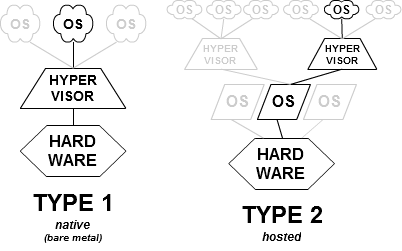
\includegraphics{Figures/hypervisor_difference.png}
\decoRule
\caption[Differences between Type 1 and Type 2 Hypervisors]{The Type 1 hypervisor, shown on the left, operates directly on computer hardware. The Type 2 hypervisor, shown on the right, is hosted on an existing operating system \parencite{Wikipedia_hypervisors}.}
\label{fig:Hypervisors}
\end{figure}

Type 1, also known as bare-metal or native. Type 1 hypervisors are run with specialised operating systems designed to give direct hardware access. This approach is generally the more efficient of the two and in some cases it can be more secure.

Type 2, or hosted, hypervisors are packaged with software that runs on a general purpose host operating system such as Microsoft Windows or general Linux distributions. Virtual machines that are run with Type-2 hypervisors are seen as processes to the host operating system. Since it shares resources with other processes that execute on the host, this is generally seen as a less efficient, but easier approach to virtualisation.

\subsubsection{Containers}

Containers are not a novel idea. Over the years there have been various isolation or containerisation techniques developed which all try to achieve secure, isolated processing environments in their own ways. These include things such as FreeBSD Jails, Linux-Vserver and Linux Containers (LXC). They are lightweight isolated spaces of resources that can be used for various things and in some cases can replace virtual machines for specific tasks. They are mainly software engines that utilise Linux kernel features in order to achieve isolation of resources and access to other processes to avoid virtualisation.

Today they are generally used to enable applications or services to be built on a variety of different system configurations without the need to worry about software dependencies. They also enable the ease of moving the application and running it on a wide variety of different systems.

\subsubsection{Differences Between Containers and Virtual Machines}

The major problem that virtual machines, henceforth referred to as VMs, have is an inherent performance hit over a single operating system, or "bare-metal" machine. Due to the implementation architecture, the hypervisor runs on or alongside the host operating system of the machine and one or more virtual machines can be created from this. Each virtual machine has its own operating system and kernel, which means that there are redundant services being executed over the machine as a whole.

Containers alleviate the resource-hungry problem that virtual machines pose by eliminating the need to run a separate instance of a guest kernel and operating system all together. Only a subset of components that make up an operating system is needed by a container, such as the libraries of the operating system image used and its own network stack, process tree, and others depending on the implementation.

The core differences between the two approaches are broken down in Figure \ref{fig:hypecont_diff}.


\begin{figure}[h!]
\centering
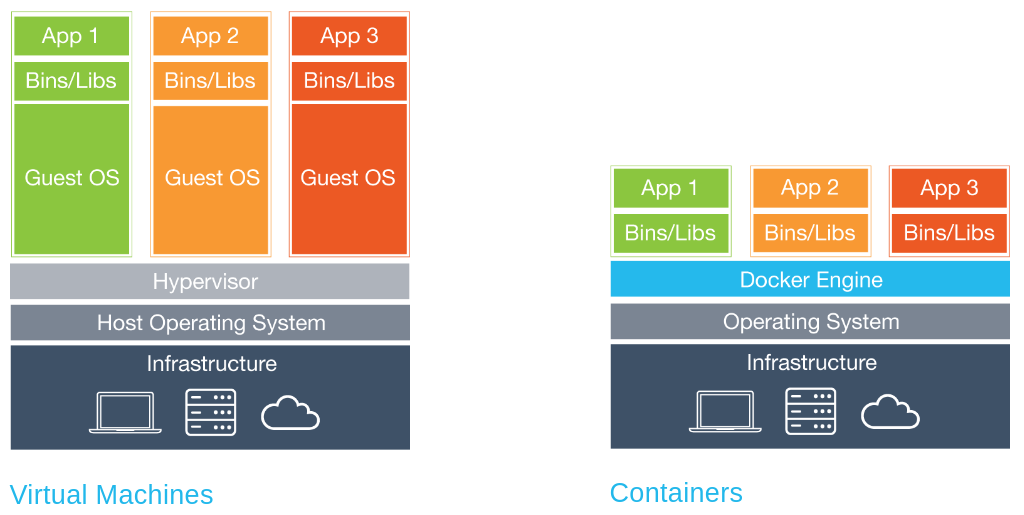
\includegraphics[width=\textwidth]{Figures/hypervisor_vs_container.png}
\decoRule
\caption[Differences between Hypervisors and Containers]{The image on the left describes the typical hypervisor-based virtual machine execution layers. The image on the right shows how container engines bypass areas of the hypervisor approach, sitting closer to the bare hardware. \parencite{enterprise_hypercont_diff}.}
\label{fig:hypecont_diff}
\end{figure}

As VMs are added to a host machine, a larger chunk of resources are reserved just for the guest operating systems themselves, leading to less resource availability for the applications or services. Not only this, but, due to the additional complexity of the VMs, they can become computationally expensive to operate in large numbers \parencite{gupta2015comparison}.

On the other hand, containers can achieve much higher density per host, that is to say that more containers can run on a single physical machine than virtual machines. Testing done for \textbf{\textit{Linux Containers and the Future Cloud}} by Rosen\footnote{Linux Containers and the Future Cloud is a presentation that was delivered for the Haifux Club at the Israel Institute of Technology on 17 March 2014. \url{http://cs.technion.ac.il/events/2014/2012/index.html}} \parencite{rosen2014linux} showed that OpenVZ and PCS achieved densities roughly 54\% and 227\% more than the best VM platform tested (RHEL KVM), respectively. 

Another advantage of containers is that the startup and shutdown time can be much faster than VMs, which can lead to higher overall time-to-business, and native nesting support (containers within containers). This is due to virtual machines needing to do the entire guest operating system boot process. However, when the working environment is of a heterogeneous nature, such as networks of systems that run operating systems other than Linux, containers can be restrictive and introduce additional complexity. Other operating system vendors have started making efforts to produce their own container systems or support existing ones, so this issue may be resolved in the future \parencite{ms_docker}.


\subsubsection{Types of Containers}

There are various container systems that are used today (\textit{vide supra}) and studies have been done to compare some of the major containers systems used in the modern world in terms of performance, features and/or security \parencite{bui2015analysis,gupta2015comparison,xavier2013performance}.

The following section mentions some of the container systems spoken about in the papers referenced above. Note that the following is not an exhaustive list of container systems nor their features.

\paragraph{Docker} \label{container:docker}
Docker is one of the most recent (2013) and popular container systems being used today. This specific one has recently enjoyed massive adoption by various types of companies and research groups, helping replace virtual machine infrastructure and creating ease of application development and deployment. It is based on LXC, another container system, but has moved from using this as its core to utilising linux control groups (cgroups) and namespaces\footnote{Control groups and namespaces are Linux kernel features that allow for isolation of resources and processes for processes.} more directly \parencite{merkel2014docker}. Docker makes use of hostname, inter-process communication (IPC), mount, network, user and process identifiers (PID) namespaces \parencite{bui2015analysis} for security and privacy as well as cgroups for resource limiting.

While it has other uses, the primary selling point of Docker is to contain a single application or portion of an application with speedy deployment. It can provide secure and robust communication between a container and its host. Each container has its own virtual network stack, unless manually specified otherwise, which takes care to abstract network traffic from the host. The organisation behind Docker provides a registry service called the Docker Hub which hosts many official and third party Docker images, which boosts the sharing capability and increases development startup time. Private registries are also available for more specialised or sensitive use \parencite{boettiger2015introduction}.

The Docker engine uses an API which allows for automation scripting and development, better management tools and reporting on containers and images. It also makes use of an abstraction layer that allows it to work on different Linux operating systems in identical fashion. To get compatibility within Microsoft Windows, Docker makes use of a hypervisor in which it gets deployed.

The main caveat with Docker is that it requires privileged user permissions on the host operating system in order for the user account to interact with the Docker system service, which takes care of launching and managing containers. This is an issue in multi-user environments.

\paragraph{Linux-Vserver} 
This is one of the oldest containerisation systems around, with the first public release in 2003 \citep{linuxvserver}. In order to use this container system, the system administrator is required to patch the host Linux kernel for their operating system in order to provide isolation between the host system and containers. This patching also enables inter-container isolation in addition to resource control \parencite{quetier2007scalability}.

It makes use of chroot calls to create a new root file system for each container\footnote{Chroot is an an isolation technique on Linux that changes the apparently root directory for a process.}. Due to the use of global PID spaces for process isolation, good performance and scalability is easy to achieve , but features such as live migration and other virtualisation features are mostly not achievable with Linux-Vserver. All containers share the same network subsystem, with identifiers added to packets to prevent snooping. This approach disallows containers from modifying their own routing tables, which may potentially limit its usefulness for tools that require unique network configurations. For CPU isolation, the Linux Scheduler is used with a Token Bucket Filter\footnote{The token bucket filter in this case is the application of the token bucket algorithm applied to the CPU scheduler.} on top of it \parencite{soltesz2007container}. Each process is linked to the creation of a token. Memory restrictions are done through rlimit, the Linux kernel system feature that controls memory usage per process or user. Recent version include cgroup support.

Linux-Vserver has proven to not be as flexible as other container systems.

\paragraph{OpenVZ}
OpenVZ is a relatively old container system, released first in 2005. It is similar to Linux-Vserver, but it uses Linux namespaces directly \parencite{dua2014virtualization}. OpenVZ treats a container as a small instance of a virtual private server (VPS) rather than as an application, as Docker does.

It uses its own custom patched Linux kernel dubbed the OpenVZ kernel which provides features such as virtualisation, isolation, resource management, and checkpointing which are common to other virtualisation platforms \parencite{kolyshkin2006virtualization,che2010synthetical}. Modern versions can use the mainline Linux kernel 3.x with a reduced feature set. OpenVZ can also be limiting to certain application due to the restrictions placed on the kernel requirements. All containers on a single host use the same kernel and architecture. Each container has its own process tree, serial ports, file system and network stack, although the host's network stack can be passed through to containers.

\paragraph{LXC}
LXC, or Linux Containers, is a newer container technology which was first released in 2008. It makes use of namespaces, in similar fashion to Docker, since Docker was based on LXC. Cgroups are utilised to provide resource management and I/O (input/output) operations are done through the Completely Fair Queuing (CFQ) scheduler \parencite{rizki2016performance}.

With some configuration LXC allows containers to be executed by unprivileged users \parencite{linuxcontainerscom}. This is especially useful in multi-user environments such as high performance computing (HPC) centers, where many users are on the same machine and have potentially sensitive information to process.

It works at a significantly lower level than container systems such as Docker, having less abstraction and in turn a steeper learning curve. This also makes it possible to achieve better performance.

\paragraph{Solaris containers/zones}
Solaris zones are around the same age as OpenVZ, being made available in 2005. It was specifically designed by Oracle to be used with Solaris OS and was offered to clients who were using the Solaris environment. 

Originally designed to improve on the administrative ease and feature set of Linux-Vserver and FreeBSD jails available at the time, it attaches zone identifiers to processes in order to limit visibility of other processes, effectively hiding a process running in one zone from another. It takes advantage of many native features of Solaris such as entitlement, limits and partitions in order to do resource management \parencite{price2004solaris}.

Its main drawback is that it can not be used with other operating system environments outside of the scope of Solaris OS. This severely limits its adoption and eliminates its use in the majority of high performance computing environments.

\paragraph{Singularity}
This is the newest major container platform, publicly appearing around October 2015. Its primary use case is aimed at computational portability. The focus for this container technology has been towards researchers and scientific application from the beginning, adopting technologies and improvements that directly improve the use of these applications within the containers. Examples of this are GPU support from within containers as well as being able to utilise technologies such as MPI natively \parencite{arango2017performance,benedicic2017portable}.

Singularity does not require special privileges to execute. This is very beneficial to multi-user environments. It also has the ability to convert Docker container images to be used in Singularity, which ensures a large range of base applications and good compatibility. Process namespace isolation is used to its fullest extent by default with Singularity and it has transparent networking. Each container shares its environment with the user that started it, which makes it simpler to use from a user perspective \parencite{xavier2013performance}. It is also integrated in various workflow software and schedulers.

% For the purpose of this work, Docker and Singularity were identified as particularly useful container systems due to their adoption and usability in scientific research. 

%----------------------------------------------------------------------------------------

\subsection{High Performance Computing}

High performance computing (HPC) is the paradigm where multiple powerful computing systems are networked together in order to run problems that are computationally expensive or that have extremely large sets of data, in more reasonable time. Software for HPC environments needs to be specifically designed with parallelism in mind, as compute is executed over various different computing hosts in the network at the same time.

These environments are provided either by a university, computing research institution, private business or the research group itself.

\subsubsection{Virtualisation in HPC}

Due to the performance overheads of virtualisation, it is not commonly implemented in serious HPC environments. Few groups have attempted to make virtualisation a viable option for HPC. A notable example of this is the group ScaleMP. Founded in 2003, their mission was to create a hypervisor that spans multiple physical machines. This allows the user to get a singular view of multi-machine clusters, by pooling resources from all of them, which could simplify writing high performance applications to only have to deal with the view of one operating system instance.

In 2014, Dell published a blog post showing their experiments with traditional virtualisation in an HPC environment by using various different scientific benchmarks. They concluded the generally accepted outcome that, given an even playing field in terms of hardware resources, virtual machines tend to perform slower than running the task on the bare machine \parencite{dell_container_perf}.

\subsubsection{Containers in HPC}

There are two main container projects that are currently considered for high performance work, namely Docker and Singularity. Docker is the largest of the two (see \nameref{container:docker} in section \ref{container:docker}), given that it is mature and has been operational for many years. The other project, Singularity, is a fairly young, but promising new container engine. Singularity is more specifically targeted at scientific workflows and has native support for HPC-specific hardware whereas Docker does not, as it is targeted more at microservices\footnote{Microservices is a software development paradigm in which a normally tightly coupled software architecture is split into multiple loosely coupled components.}. However, due to Docker being more mature it has also amassed a large number of pre-built scientific containers that can easily be downloaded from the Docker Hub registry. Singularity is especially attractive for the HPC space due to it not requiring elevated privileges to run software, reducing security concerns, and its ability to support Docker images.

Docker has made a significant impact on the Linux developer community with the ease of building, shipping and managing software dependencies in applications. However, as had also been expressed that this "revolution" \parencite{jacobsen2015contain} has yet to make a meaningful impact on the high performance computing community \parencite{yu2015building,xavier2013performance}.

Aside from the benefit of having software dependencies that are easier to manage by packaging the specialised software into container images, there are more low level advantages to using a container approach to building software for HPC clusters. Software containers can allow performance levels much closer to a bare-metal system than a virtual machine with a hypervisor can, which makes it very attractive from a compute standpoint. In the white paper\footnote{A white paper in the technology industry is a technical document that describes how a technology or product solves a particular problem. \url{http://www.investopedia.com/terms/w/whitepaper.asp}} \textbf{\textit{Containerization of High Performance Compute Workloads using Docker}} by Christian Kniep \parencite{kniep2014containerization}, it was found that it is even possible to achieve better performance in a Docker container than the bare-metal operating system it resides on in some cases, due to different libraries being used by the container operating system.

A prototype Docker-powered HPC Cluster has also been designed and implemented, spread over different physical machines, making some modification to the network bridge to get them to work together. It was deemed feasible to implement such a system and should be considered for future work management/orchestration engines and friendly graphical interfaces \parencite{yu2015building}.

Due to the ability to wrap workflows and work environments into a highly portable package, these container technologies also become attractive as they reduce the work necessary by system administrators and managers in order to ensure that user software dependencies are met.

\subsubsection{Research}

HPC environments are generally suited to a limited set of work. Massively parallel-capable tasks benefit greatly from the services that these centers provide to their users. The current model of HPC for researchers dictates that there must be at least one system administrator available on the project who installs and manages software that is approved for use with the institution. Users are able to request software that they wish to use for installation, but there is no guarantee that it will be supported by the HPC centre. Other than using official support channels in order to support researcher workflow or pipeline, there is no way to engage with the system and make changes required by the researcher. HPC centers are generally considered to be restrictive.

%----------------------------------------------------------------------------------------

\subsection{Cloud Computing}

Before common availability of the internet as we know today, companies used to buy and maintain mainframe computers that were tasked with all the business-supporting activities that could be programmatically represented. This moved into distributed computing where multiple machines would be bought and networked in order to perform tasks together. Organisations began to offer computing time on their own servers to other parties for a price, this developed into what is known today as cloud computing. 

In layman's terms, computing infrastructure is hosted by a company or organisation and provided to end-users through an abstracted interface, known as Infrastructure as a Service (IaaS). Most cloud providers will offer one or more types of services, such as Infrastructure, Platform or Software as a Service. Each of the services offer varying levels of access to the operating system environment directly, with IaaS offering the closest to actual server access. The purpose of this is to allow people to make use of hardware infrastructure without the need to provision, manage or maintain them physically.

\subsubsection{Micro-cloud}

A relatively new paradigm, "micro-cloud" or "micro-clouds" is bringing the idea of shipping code, or applications, instead of data to be processed at different locations. The paper \textbf{\textit{Mobile Micro-Cloud: Application Classification, Mapping, and Deployment}} \parencite{wang2013mobile} defines a micro-cloud as a "logical network" which consists of two main parts. The first is a "core" or central platform where the data set to be processed resides in its entirety. The second part consists of one or more "edge" platforms or small segments of computing power scattered across different locations, internally or externally, which deal with a need-to-know base of information from the core which is required for computing the task given to it.

The term "micro-cloud" was spawned from the paradigm of cloud computing, and describes the shift from using infrastructure hosted at and owned by a particular institution to using the infrastructure of another company over the internet. In this model an organisation does not pay for the installation cost and maintenance of hosting physical servers, instead they pay a monthly or sometimes yearly rate to a cloud computing provider such as Google or Amazon.

Security concerns arise with data being processed in areas that are possibly not owned by the data-holder. A good security model for the data needs to be available in the system as to prevent leaking of sensitive information. An authorisation and authentication system is also important for scenarios where specific people are allowed specific access to data. 

\subsubsection{High Performance Cloud Computing}

High Performance Cloud Computing, or HPC2, is an emerging trend. Cloud computing is becoming increasingly viable for some types of research, as the pay-as-you-use model offers some real value over the need to have a physical set of hardware at the institution. Any research that requires the processing of large or many data sets have the potential to benefit from this approach as cloud providers provide powerful virtual environments that are more catered to compute-heavy workloads. It also allows the flexibility and freedom of full control over the software stacks used. Some modern cloud computing providers are offering "Cluster Computing Instances" or high powered virtual machine instances that are connected to high speed interconnects. This model has proven viable for many types of research computing \parencite{hazelhurst2008scientific}.

Research has shown that HPC2 offerings are not yet on par with non-virtualised physical high performance environments \parencite{jackson2010performance}, so there is still work to be done in order to bridge the gap between purely virtualised cloud computing providers and high performance bare-metal machines. Projects have emerged in attempt to address some of the issues with access to high performance devices for virtualised environments, one such being a novel approach to using high speed compute cluster network interconnects in a cloud environment \parencite{mauch2013high}.

\subsubsection{Issues With Cloud Computing in Research}

There are various reasons why an organisation would not be able to use a conventional cloud computing platform to provide their products and/or services. Running costs, internet access, scale or privacy issues of using the cloud are among some of the reasons an organisation's internal ability to manage those aspects may outweigh the attraction of use.

Smaller organisations benefit greatly from utilising the offerings of cloud environments due to the high cost of infrastructure acquisition, but subscription costs for storage and compute will continue to grow as time progresses. The potential to become more costly to maintain a cloud environment than a physical one increases when organisations want to scale their services or utilisation. Some flexibility is also sacrificed as users have no physical access to any of the hardware that they are renting, which results in users having to work around restrictions or limitations that are in place with cloud environments. This issue is constantly being worked on by cloud environment providers by offering increasing amounts of customised solutions for various use cases as evident by regular releases of new platforms and tools by said providers\footnote{The work being done by the three most successful cloud computing provides can be found at the respective blogs: Google (\url{https://cloudplatform.googleblog.com}), Amazon (\url{https://aws.amazon.com/blogs/aws/}) and Microsoft (\url{https://azure.microsoft.com/en-us/blog/}).}.

Privacy is another fairly serious concern with cloud environments. When data is stored on cloud environments, the user is subject to the privacy policy and terms of use of the cloud provider. The user is also subject to housing the data they wish to store on one or more of the physical locations that a cloud provider may offer. Data centers are not available in every country or continent. This has potential ramifications for data that is governed with strict policies, where there is no strict control of how data is stored and/or replicated by the cloud provider \parencite{abouelmehdi2017big}. Lawmakers are catching up to the notion of privacy-centric data and location agnostic cloud environments \parencite{gholami2016big}. Researchers themselves can take preventative steps to protecting their data as well with approaches such as data segmentation, encryption and anonymity masking \parencite{sun2014data}. Unfortunately there is no concrete solution to data placement laws, short of having cloud providers open data centers in every country in the world.


%----------------------------------------------------------------------------------------

\subsection{Workflow Languages}

Bioinformatics data often needs to go through various steps of transformation to be usable for different purposes. While some pipelines or workflows are presented and shared as a structured set of tools that need to be executed in a specific order, many researchers chain tools together in novel ways to achieve their own goals. A large percentage of students and researchers in this space are not programmers \parencite{mesirov2010accessible}. Many researchers and students in the field of bioinformatics perform data analysis by using programming languages including, but not limited to Python, R, or Bash to write scripts that are highly specific to the tools, data and environment that they are working on. There is a growing problem with these pipelines not being easily reproducible or extensible by others. Implications of this are that it becomes difficult to verify whether the results of other researchers are correct and to expand on the groundwork that others may have laid with their original work.

Workflow languages offer a way to address this issue. They provide a structured way for researchers to provide the inputs, tools and outputs that are required for each possible step of an analysis. The execution tools for the specific languages allow these workflow definitions to be executed on different machines without needing to modify them for your specific environment and consequently make it significantly easier to acquire the specific tools and versions of those tools for the said workflow. Many of these workflow languages also integrate with container technologies such as Docker and Singularity to retrieve the desired tools at the time of execution.

The following is a non-exhaustive list of actively developed workflow languages and standards that are used in the bioinformatics space.

\paragraph{Common Workflow Language} The Common Workflow Language (CWL) describes itself as a standard or specification for defining computational workflows. CWL does not provide an all-in-one solution to executing workflows, but rather attempts to provide the common base that future workflow execution systems could use to define the tasks to be done\parencite{amstutz2016common}, providing support for popular tools and services such as Docker containers. The CWL standard is implemented in various workflow execution tools such as cwltool\footnote{\url{https://github.com/common-workflow-language/cwltool}}, Arvados\footnote{\url{https://arvados.org/}}, Toil\footnote{\url{https://github.com/DataBiosphere/toil}}, Galaxy\footnote{\url{https://galaxyproject.org/}} and other.

Cwltool is the reference implementation of an interpreter for the CWL standard that provides the common base set of features that is expected from a tool that implements said standard. It is up to the tool which implements the standard to add additional functionality such as parallelism and utilising cloud environments.

\paragraph{Nextflow} Nextflow is a workflow or pipelining language with Linux as its primary focus and Docker containers as a first class citizen, later also adding support for Singularity containers. Users of Nextflow are able to describe their data processing pipeline in the Groovy programming language. This tool allows users to describe their workflow and execute it on a variety of platforms such as traditional HPC scheduling systems or public clouds such as Amazon Web Services or Google Cloud \parencite{di2017nextflow}.

While using this tool means that users will have to conform to its requirements, such as knowing Groovy, it provides many other benefits such as portability, fault tolerance, reporting and support for container scheduling systems all in one packaged solutions. A prototype for converting CWL specification to Nextflow instruction was in development at some point, but was cancelled\footnote{\url{https://github.com/nextflow-io/cwl2nxf}}.

\paragraph{Snakemake} The Snakemake workflow management system uses Python as a language to describe workflows. This makes it attractive from an ease-of-use perspective as Python is considered a relatively simple and efficient language to use for non-performance oriented scientific purposes\parencite{rashed2012python,muller2015python}.

It provides features such as visualisation of the workflow, exporting to CWL and executing workflows on the Google Cloud specifically. Snakemake also provides support for container technologies such as Docker and Singularity, but has an added advantage of being able to utilise the Conda\footnote{\url{https://conda.io/en/latest/}} distribution service for Python natively. This adds additional flexibility to the user. It provides support for HPC schedulers through a relatively simplistic method of passing the job as a Linux shell command, which makes it relatively compatible with most common schedulers.

\section{Project Aims}

There are three main research questions that this project aimed to address. The overall aim was to address these issues by providing an automated tool and simple interface for researchers to utilise the cloud for their specific needs, without the need for complicated dependency management, manual administration or technical knowledge.

\subsection{Is it feasible to move workflows/pipelines to the cloud?}
This questions tries to understand if the paradigm of moving researcher workflows to remote locations is feasible or not. This is the main focus of this project and the subsequent questions rely on this main question.

\subsection{Can the cloud environment be simplified for researchers?}
It is unreasonable to expect that most researchers understand how to use specific technologies such as cloud computing environments and specific operating systems, along with their intricacies, in order to reproduce their working environment remotely. Therefore, the remote execution environment should be simplified for use by non-technical researchers by attempting to create a structured and reproducible way for them to define their specific environment which can automatically be made for them.

\subsection{How can workflow languages be supported in the cloud?}
Standards need to be put in place in order to create redistributable workflow specifications. It is difficult to maintain a system that supports endless different workflow specifications. A balance needs to be struck with how many to support. This question asks how workflow specifications can be integrated into a cloud environment to allow for reproducible science and researcher flexibility.

The source code for the prototype software developed for this project can be found at \url{https://github.com/Banshee1221/Nikeza}.
% Chapter 1

\chapter{Methodology and Requirements} % Main chapter title

\label{Chapter2} % For referencing the chapter elsewhere, use \ref{Chapter1} 

%----------------------------------------------------------------------------------------

% % Define some commands to keep the formatting separated from the content 
% \newcommand{\keyword}[1]{\textbf{#1}}
% \newcommand{\tabhead}[1]{\textbf{#1}}
% \newcommand{\code}[1]{\texttt{#1}}
% \newcommand{\file}[1]{\texttt{\bfseries#1}}
% \newcommand{\option}[1]{\texttt{\itshape#1}}

%----------------------------------------------------------------------------------------

\section{Background}

As Figure \ref{fig:traditional_data_model} demonstrates, the traditional way for researchers to process data which they do not produce themselves or already possess is to first transfer the data from a remote holding source to themselves. This process is almost always the bottleneck in data processing as large data sets can take a large amount of time to retrieve. This is a growing issue and will continue to become more serious as time progresses and data sizes increase. As such, data processing capabilities should ideally be made more readily available at institutions that generate and/or carry large data sets to offset the amount of time wasted in transferring such data.

\begin{figure}[ht!]
\centering
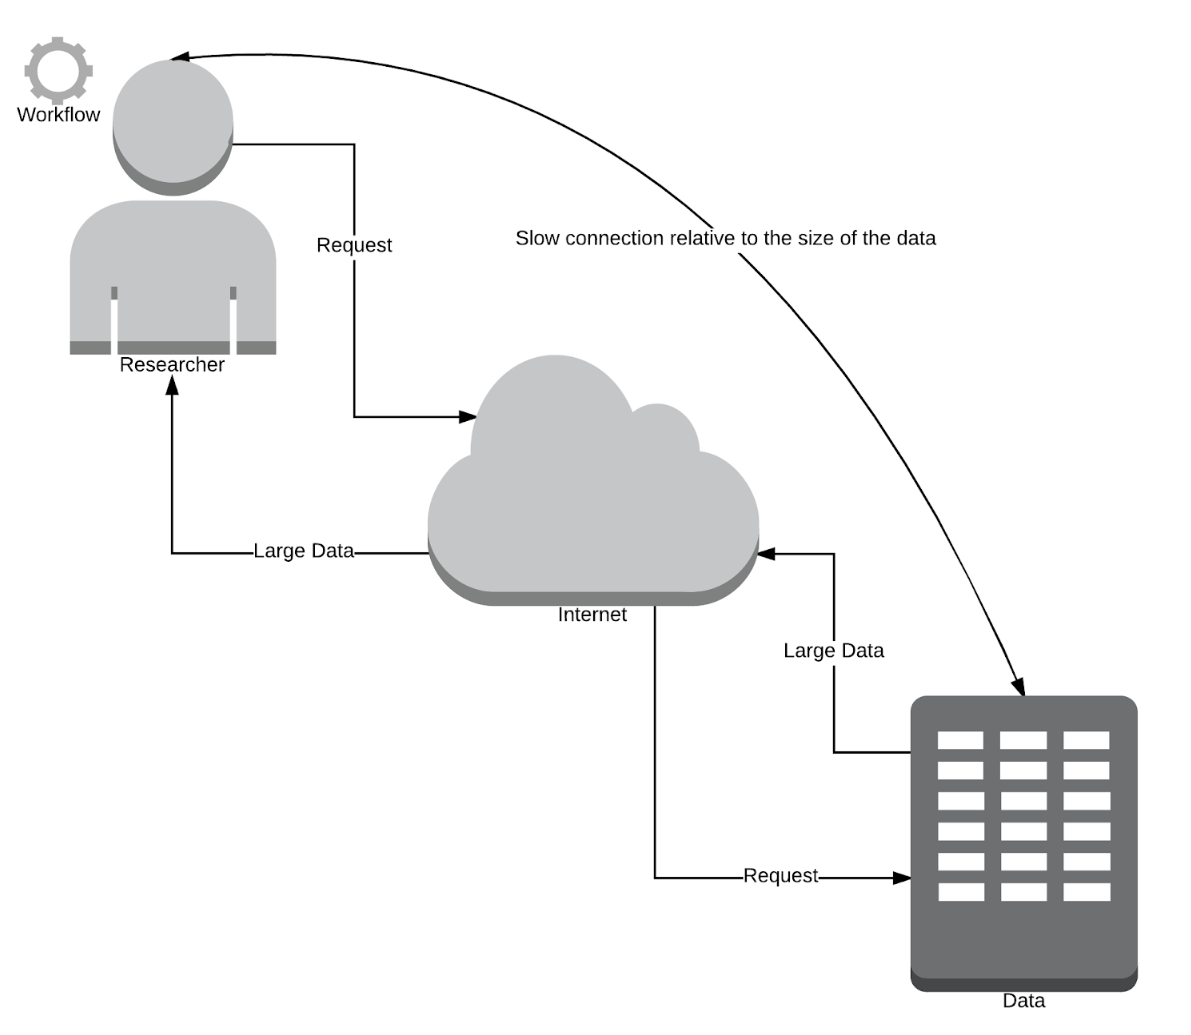
\includegraphics[width=\textwidth]{Figures/traditional_processing_model.png}
\decoRule
\caption[Traditional Researcher Data Usage Model]{This figure demonstrates how a researcher typically interacts with a remote data set. The data is transferred to the researcher via the internet in most typical environments, unless the data can be acquired through offline modes such as couriering.}
\label{fig:traditional_data_model}
\end{figure}

%----------------------------------------------------------------------------------------

Various methods for processing large data currently exist. Many of these solutions have been attempted at academic institutions such as the South African National Bioinformatics Institute at the University of the Western Cape. The next section describes some of these methods along with some advantages and disadvantages of each method.

\subsection{Traditional High Performance Computing Centers}

Processing of data at high performance computing institutions via data transfer through the use of the university network is common among research institutions where spending large amounts of money on computing resources is not a priority. Most research institutions rely on nationally available computing organisations, such as the Center for High Performance Computing (CHPC) in South Africa, to process data sets generated by their research. These organisations can be private sector businesses, government funded initiatives or a combination of the two.

HPC centres can be a viable option if the organisation offering the computing resources is not oversubscribed, has good availability and if the data set is not too large. Time may become an issue when data sets reach larger sizes, resulting in transfers that may take an unrealistic amount of time.

The CHPC is a part of the Council for Scientific and Industrial Research (CSIR)\footnote{\url{https://www.chpc.ac.za}} and provides access to two fairly powerful clusters. The main offering is the Lengau Cluster, which is a petascale system that is offered with time sharing and/or resource sharing options. They also provide access to a GPU cluster which some scientific workflow may call for.

While this has done much to aid the research tasks of various academics in the country, the CHPC is plagued with various non-user friendly issues and downtime which interfere with the researcher's deliverables.

\subsection{Inter-university Data Processing}

Universities often have very high speed networks that interconnect them nationally. In South Africa, the Tertiary Education and Research Network (TENET) of South Africa operates an internet exchange named the South African National Research and Education Network (SANReN). This network offers high speed 10 Gbps fibre channels to various universities that are involved with the project.

Researchers may be working on projects that span multiple universities. In these cases, and sometimes others, universities will provide computing resources to researchers that they are in collaboration with. The research data will either already be housed at the institution that a researcher is collaborating with or the data will need to be transferred to this university. This again could prove to be a problem if the data volumes are too large to transfer in a reasonable amount of time.

\subsection{Physically Moving Data Drives}

As previously mentioned, it is possible for data that needs to be processed to be too large to move due to reasons such as slow network speeds or data sizes that are too large. If a research institution does not have the necessary computing resources they may resort to physically moving the data that they wish to process to locations that have the ability to do so \parencite{marx2013biology}.

Utilising this method of data movement has major risks. The physical security of hard disk drives in transit can often not be guaranteed. This issue becomes compounded when the data in question is sensitive and has policies surrounding who is allowed to use it and where it is allowed to be sent.

\subsection{Utilising the Public Clouds}

Modern cloud computing offers a wide range of tools for end users to create environments to suit their needs. By offering various solutions such as Infrastructure as a Service (IaaS), Platform as a Service (PaaS) and Software as a Service (SaaS) research institutions can choose a model for data processing that fits well into their budgets. Often, a plan is chosen that allows an institution to have a chunk of storage, such as Amazon's S3, provided by the cloud provider. Data must be transferred to the cloud storage solution, after which it will be accessible from virtual machines that are created on the cloud.

This solution makes the management of hardware resources significantly easier for institutions, due to no physical hardware being owned. It also often provides more flexible computing resources as CPU, memory and disk can easily be scaled up at an additional cost with most providers.

Utilising this approach can lead to increased issues with network related activities if data volumes are large. This is mostly due to the outbound internet connection that is available in the country. The SANReN network provides a significantly faster connection locally between universities than internationally. Since most well-established cloud providers keep their data centers outside of Africa\footnote{This is true at the time of writing, but it has become evident that more cloud providers are interested in providing computing and storage resources located in South Africa \parencite{aws_sa,azure_sa}.}, the time taken to send raw data will increase substantially.

Ignoring the issues mentioned above, one major impairment to the use of cloud computing is the lack of scientific software and tools that work natively with these environments. Many scientific applications do novel operations which need to be individually catered for \parencite{barga2011bioinformatics}.

\subsection{Local Computational Ability}

Research centers, such as SANBI, may offer a local storage and compute cluster that can be used to process research data. This would be the ideal solution for most research institutions in terms of data transfer as it reduces potential problems with politics and policies surrounding certain types of data and allows quick feedback and local support. However, this requires that institutions have a large initial capital in order to purchase all the equipment needed. Once the initial setup is complete, additional expense goes towards the maintenance of the cluster as well as paying the salary of a technical officer to oversee the operation and maintenance of said cluster.

% New approaches are being attempted in order to simplify the processing of data while reducing the need to move it. This would appear to be a good solution to the issue of growing data volumes if each institution possessed the compute ability to process it all. Due to this, the next logical question to ask is whether processing can be done at the location of the data, rather than to move it before hand. This has prompted the creation of various solutions, one of which is mentioned below:

\subsection{Semi-Private Research Clouds}

Formerly known as the African Research Cloud (ARC), the South African Data Intensive Research Cloud is an inter-university research cloud project. The goal of this project is to bring storage and compute needs to Southern Africa (as well as Africa) as a whole, with each university providing parts of these services. The end user, or researcher, will be provided with a singular cloud interface with which they can create virtual compute instances and utilise data or provide their own, where the system would be intelligent enough to ensure the user is provided the resources from the centre closest to the data. The primary focus of this initiative is to support astronomy and bioinformatics workflows.

There are other project like this which aim to provide researchers in various regions and fields with flexible compute capabilities without requiring the funding to purchase and maintain physical infrastructure or make use of the more limiting HPC centers. These include the UK based Cloud Infrastructure for Microbial Bioinformatics (CLIMB) system \parencite{connor2016climb} and the Australian based National eResearch Collaboration Tools and Resources (NeCTAR) research cloud \parencite{nectar_cloud}.

\subsection{Tool Wrappers and Workflow Generators}

Projects such as the Galaxy platform introduce a visual web-based platform and extensive framework for bioinformaticists to work with tools in the field \parencite{afgan2016galaxy}. It aims to provide a way to string tools together into workflows by having tool definitions written for each piece of software and then manipulating their inputs and outputs in the context of other tools from a web interface.

It is a collaborative effort between the group that make the core service as well as the community that build the integration for it with the tools that bioinformatics researchers typically use. This approach not only allows easier consumption of larger sets of data, but also fundamentally encourages the sharing of analysis. The caveat with Galaxy is that the end-user, the researcher or academic, is restricted to using the toolset that is provided with that instance of Galaxy, whether that be the public Galaxy instances such as \url{https://usegalaxy.org}, or a Galaxy instance that is available at the researcher's institution. Software can be added, but it is a similar process to maintaining software in the traditional cluster computing way.

The Galaxy project is actively developing technology that allows this platform to sit on top of cloud environments in order to take advantage of the flexibility that they provide. Dubbed CloudMan, the project aims to enable better usage of resources and allow the project to be run on more platforms \parencite{afgan2012cloudman}. This technology is similar to other infrastructure-as-code tools such as Terraform\footnote{\url{https://www.terraform.io/}}, but it is built with a focus on compatibility with the Galaxy project.

This project is a good example of what could be used at an institution to provide analysis tools to process data that exists at the institution, provided that the software requirements are well defined by the researchers.

%----------------------------------------------------------------------------------------

\section{Project Requirements}

With respect to the research questions posed above, this thesis presents a proof-of-concept solution in the form of Nikeza. Nikeza, meaning "give away" in isiXhosa, will be a software product that compliments an existing cloud or container provisioning and orchestration environment through a plugin system. It will act as a management add-on that is written mainly in the Python programming language, specifically Python version 3, which allows it to run on most modern computing environments and operating systems. Plug-ins will be easy to write and theoretically allow many different virtual provisioning environments to utilise Nikeza.

A web application will be provided to allow users to upload their workflow document and select data from the provider's databases. The end user will also be shown updates to how their tasks are performing and when they are complete. User generated output will be moved to specific locations so that they may be retrieved by the user afterwards.

A backend service will be responsible for translating the user input from the web interface into commands that are understood by the platform that is being used at a given institution.

\subsection{System Context}

The assumption is that an institution will already be running a cloud environment and Nikeza will interface with the existing system in order to give it commands for correct execution based on the user input.

As Figure \ref{fig:existing_provider_environment} shows, the premise is that Nikeza would sit as a service which complements an existing storage and cloud infrastructure. A web interface is presented to a user with various options regarding which data he or she needs to access in order to do processing on, the location of the output data and options to upload their own workflow blueprint to the server. Once the user has submitted this, the Nikeza system translates their workflow blueprint into commands that are understood by the existing infrastructure. The user will receive periodic updates on the process of their workflow execution.

While there are other potential tools and services that could achieve similar results, a cloud environment is used due to the growing popularity of the cloud storage and computing ecosystems in the biomedical space \parencite{navale2018cloud,connor2016climb,afgan2015genomics,liu2014cloud}. Along with this, utilizing a cloud environment affords the potential for many aforementioned tool and services to be implemented on top of it with a more streamlined and integrated, single-access perspective.

\begin{figure}[ht!]
\centering
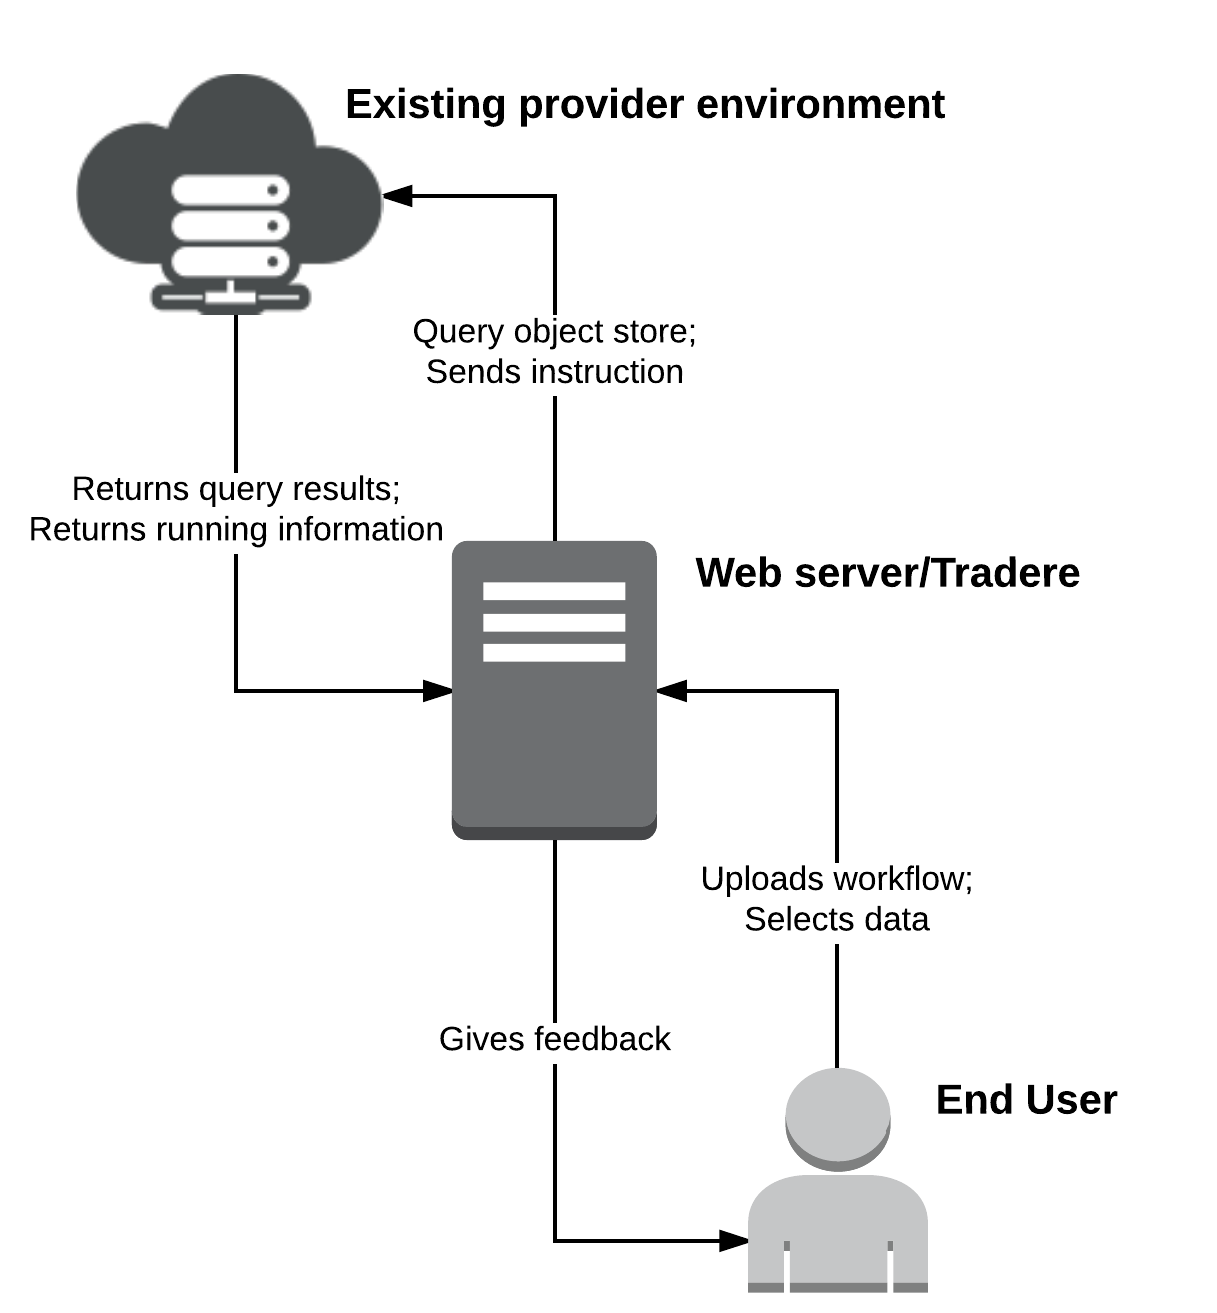
\includegraphics[width=\textwidth]{Figures/2_existing_provider_environment.png}
\decoRule
\caption[Nikeza System Context]{This figure demonstrates the concept that powers the implementation of the Nikeza project.}
\label{fig:existing_provider_environment}
\end{figure}

\subsection{Use Cases}

This section details use cases, or applications, for the proposed software system.

\subsubsection{Analysing data that is too large for a researcher to retrieve in reasonable time}

With growing data set sizes, it may not always be feasible for a researcher to wait for the retrieval of a set of data that they wish to analyse. In this case, a researcher may be able to define a workflow of the analysis that they wish to perform on data as if it were with them locally and move that definition to the environment which hosts the data. The workflow definition is understood by the remote environment and used to create a portable workflow execution environment using virtual machines and Docker containers.

Since the data already exists at the remote location, making a copy of the data set for the execution environment  or potentially, though unlikely, using it directly is objectively faster than first waiting for the data to be retrieved by the researcher. Multiple data sets may also be chained in a workflow definition, provided that all data sets exist at the remote location and are accessible to the user.

Once the execution environment completes its given objectives, the resultant data is moved off of it and onto the remote environment's storage, where the researcher is able to retrieve the completed analysis results. This could result in significantly smaller download sizes as the results of an analysis tend to be smaller than the data set itself.

\subsubsection{Sharing results of large analyses with others}

In some cases, the results of an analysis or analysis chain can be very large itself. This is seemingly counter-productive to the intended solution offered through this project. However, it is possible that collaboration efforts could lead to one researcher not actually needing to work with the results of said analysis.

In this case, one researcher would execute their analysis against a remote data set(s) and the results of that would be used by another researcher which is either closer to the data or able to execute their own analysis or analysis chain on the results of the previous.

\subsection{Conceptual Model}

The conceptual model details the components of the software architecture. This section will present the overview of the system model.

Figure \ref{fig:sytem_concept} showcases the interaction of the user and the system, as well as the various system components. This is the overview model for how the user interacts with the system and how the system responds based on the user interaction.

\begin{figure}[ht!]
\centering
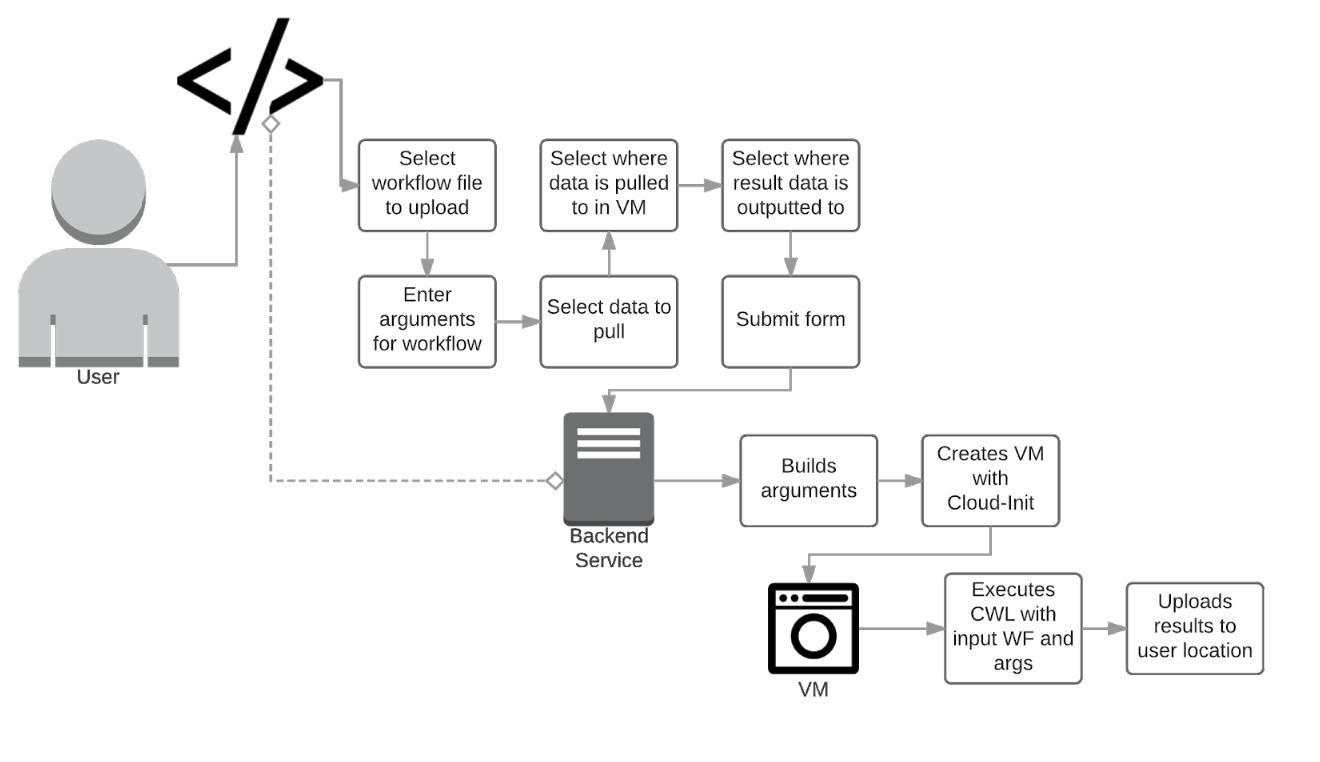
\includegraphics[width=\textwidth]{Figures/2_conceptual_model.png}
\decoRule
\caption[Nikeza System Concept]{This figure overviews the conceptual interaction model for the user and the project.}
\label{fig:sytem_concept}
\end{figure}

\subsubsection{User}

The user is able to navigate to a web interface that is provided by the project system. When first visiting this, the user is presented with a login screen so that they may authenticate against the backend system that is being used by the Nikeza system. The credentials of said user are stored with a unique cookie in the browser and on the Nikeza system side, after which they are then presented with a queue of current jobs belonging to their account. The user can select to create a new job or stop one that is already in progress. The user is also presented with a view which allows the selection of data from the backend.

\subsubsection{Nikeza System}

The project system is hosted on a public facing web server which is located near the backend cloud environment that is in use. It directly engages with the user and the cloud environment, acting as a middle man for both. The project takes care of translating user commands into instructions for the backend environment and does routine checks on jobs running for each user.

\subsubsection{Cloud Environment}

The cloud environment handles the majority of the work and takes care of running the actual analyses. It is responsible for creating virtual machines on demand, in order to accommodate the user workflow. The Nikeza system injects the workflow from the user into a newly created virtual machine and data is mapped from the storage environment into the virtual machine. Once processing is completed, the results are moved from the virtual machine into the storage environment and the virtual machine is destroyed.

\subsection{Architectural Detail}

As shown in the conceptual model (Figure \ref{fig:sytem_concept}), there are many different parts of the system that work in sequence to give the user the results. Figure \ref{fig:system_detail} expands on this and describes the complete interaction model of all the components in the system.

\begin{figure}[ht!]
\centering
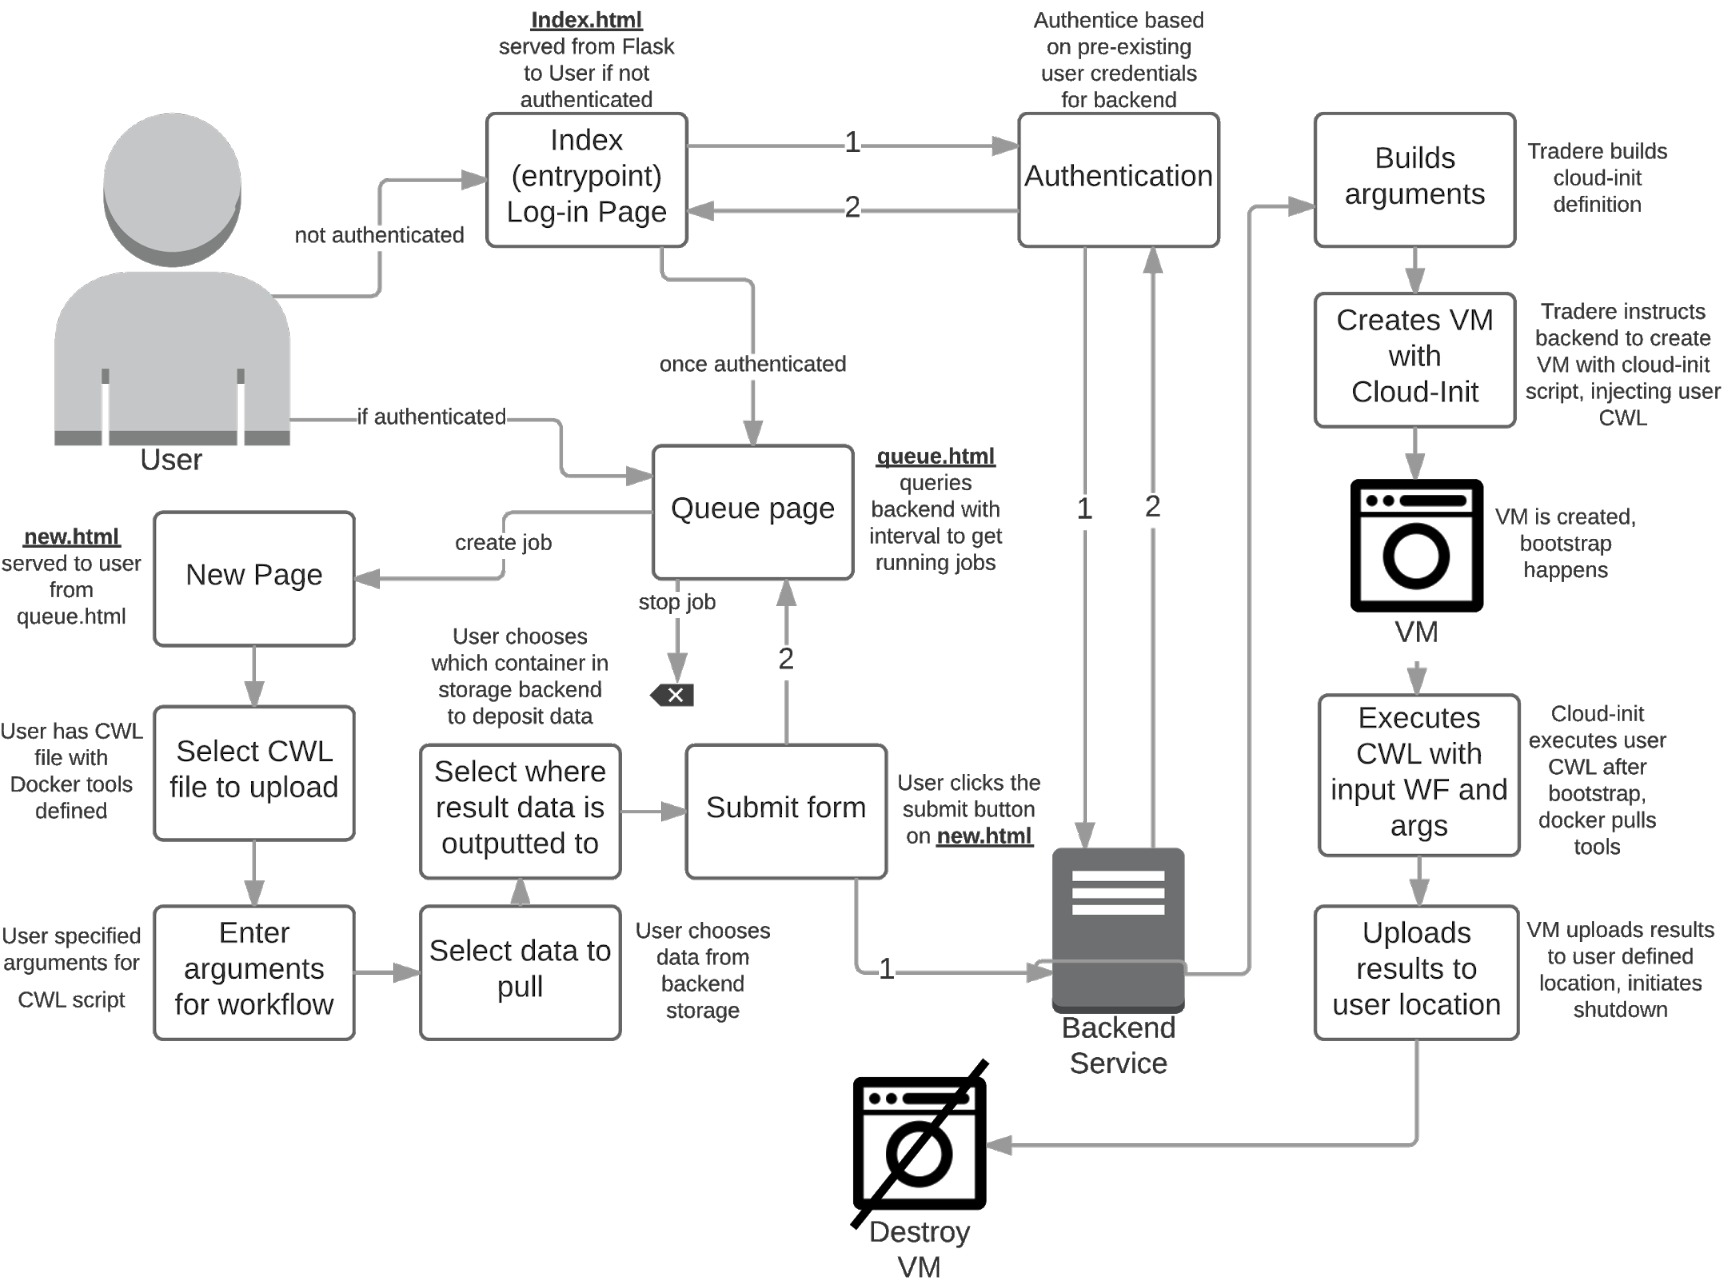
\includegraphics[width=\textwidth]{Figures/2_detailed_model.png}
\decoRule
\caption[Detailed Nikeza System Model]{This figure details the interaction model of components and the user in Nikeza. Most of the interaction behind the user-facing components are not exposed to the user and are automated.}
\label{fig:system_detail}
\end{figure}

 A new user must authenticate with the system before they can interact with it. This is done through the credentials of the cloud backend that the system is using, OpenStack in this case. The user would be provided these credentials from the institution that they want to use or from some federated authentication platform if supported. If the user has already authenticated with the system then they are not required to log in again. The Nikeza system merely tries to pass the credentials that the user supplies it through to the backend cloud environment to try to authenticate. If this fails (e.g. incorrect user credentials) then the user is presented with an error message and given the chance to try again.

The landing page for a logged-in user is the queue of jobs. This page queries the backend system for a list of jobs that may be running for that user (jobs that they have created and that are running). On this page the user can select job entries, if there are, and choose to stop the execution or they can select to create a new job. If the user selects to stop a job, an instruction is sent from the Nikeza service to the cloud platform (backend service) in order to destroy the virtual machine with the given job ID. If the user selects to create a new job they are redirected to a page that presents them with options for a new job.

The new job page will present various options for the user. These options are mandatory for submitting a new workflow and include:
\begin{itemize}
    \item Uploading their workflow definition file;
    \item Providing the arguments that the given workflow file expects when executed;
    \item Selecting the data they want to process (which is presented to them given they have access to the data through security policies/profiles);
    \item Select where the data-to-be-processed is pulled into and the resultant data is generated on the virtual machine that will be created for their workflow;
    \item Select where the resultant data is uploaded to on the backend service. 
\end{itemize}

The user can then select whether to start the job or to cancel and return to the queue without adding the new job. If the user selects to start the job, the workflow definition is uploaded from their computer and, along with all the parameters that the user filled in, an instruction log is generated by Nikeza. A virtual machine creation is requested by Nikeza and the instruction log is specified to bootstrap the creation of the virtual environment. In the meantime, the user is redirected to the queue page, where they can see the status of the virtual environment that is running their workflow. Once the job is completed in the virtual machine the data is moved to where the user specified and the virtual machine is destroyed, removing it from the queue page, and the user can retrieve the data by logging into the backend dashboard.

\subsection{Technical Functionality Requirements}

The overall goal of Nikeza is to provide an easy-to-use interface for end-users to submit their workflow to a cloud environment in which some research data is located in order for their workflow to be executed with minimal interaction. The functionality below provides the ability to answer the research questions being asked in this thesis.

\subsubsection{Allow users to execute scientific workflows without needing technical expertise}

The user's workflow submission must be understood by the system and automatically executed without leaving things behind on completion. It should be fully automated.

\subsubsection{Allowing users to execute scientific workflows on data that does not exist locally}

The user must be presented with a list of data, which they would have access to through pre-specified policies. They must be able to select the data that they want to do processing on.

\subsubsection{Allowing the system to run without modifying existing backend environments}

Nikeza must be designed in such a way as to allow the existing backend setup to stay intact, with minimal to no changes required by administrators. 

\subsubsection{Easy-to-use, human friendly user interface for the web application}

The user must be presented with an easy to understand, human friendly web interface which has all the technical details and commands abstracted.

\subsubsection{Simple plugin system in order for providers to be able to easily adapt Nikeza to their environment}

The application should support different environments through a translation plugin system in which the administrator of a system can write the needed operations in order to support their system. 
% Chapter 1

\chapter{Implementation} % Main chapter title

\label{Chapter3} % For referencing the chapter elsewhere, use \ref{Chapter1} 

%----------------------------------------------------------------------------------------

% % Define some commands to keep the formatting separated from the content 
% \newcommand{\keyword}[1]{\textbf{#1}}
% \newcommand{\tabhead}[1]{\textbf{#1}}
% \newcommand{\code}[1]{\texttt{#1}}
% \newcommand{\file}[1]{\texttt{\bfseries#1}}
% \newcommand{\option}[1]{\texttt{\itshape#1}}

%----------------------------------------------------------------------------------------

This project followed a non-standard approach to software development which incorporated aspects of various software engineering standards. The general approach to implementation followed the design philosophy of dependency injection.

The scope of this project involved conceptualising and designing a software system as well as implementing a working prototype of said software for a specific virtualisation platform. Three high powered computer servers were used to build up the hardware environment. In this instance, OpenStack was chosen as the appropriate provider environment. OpenStack is industry-ready software that is currently being utilised for cloud projects in academia around South Africa, such as with the Inter-University Institute for Data Intensive Astronomy (IDIA) and South African Data Intensive Research Cloud (SADIRC), previously known as the African Research Cloud (ARC).

\section{Backend}

\subsection{Hardware}

Decommissioned hardware from the Physical Science department was donated in order to be used for e-research efforts at the University of the Western Cape. Some of the hardware donated was utilised for this project. Table \ref{tab:hardware} details the hardware specification.

\begin{table}[ht!]
\caption[OpenStack Server Hardware Specification Table]{Hardware specification of the servers used to host OpenStack.}
\centering
\label{tab:hardware}
\resizebox{\textwidth}{!}{%
\begin{tabular}{p{0.15\linewidth}p{0.2\linewidth}p{0.2\linewidth}p{0.15\linewidth}p{0.15\linewidth}p{0.2\linewidth}}
\toprule
Description    & Physical Device           & CPU                                  & Memory                           & Storage            & Network                                                                                                     \\ \midrule
Controller & Supermicro CSE-512F-350B  & AMD Opteron 4334 - 6 cores @ 3.1GHz  & 64GB Samsung DDR3 @ 1600MHz ECC  & 223.6GB RAID1 SSDs & \begin{tabular}[c]{@{}p{1\linewidth}@{}}x4 Intel I350 Gigabit Network Connection;\\ x2 10-Gigabit X540-AT2\end{tabular}  \\
Compute             & Supermicro AS-2042G-72RF4 & AMD Opteron 6348 - 48 cores @ 2.8GHz & 256GB Samsung DDR3 @ 1600MHz ECC & 13.7TA RAID5 HDDs  & \begin{tabular}[c]{@{}p{1\linewidth}@{}}x4 Intel I350 Gigabit Network Connection;\\ x2 10-Gigabit X540-AT2\end{tabular} \\
Storage             & Supermicro AS-2024G-72RF4 & AMD Opteron 6348 - 48 cores @ 2.8GHz & 256GB Samsung DDR3 @ 1600MHz ECC & 13.7TA RAID5 HDDs  & \begin{tabular}[c]{@{}p{1\linewidth}@{}}x4 Intel I350 Gigabit Network Connection;\\ x2 10-Gigabit X540-AT2\end{tabular}  \\ \bottomrule
\end{tabular}%
}
\end{table}

Other than the server hardware, two network switches were utilised. One switch was used for internal university network access as well as management and operated at 10 Gbps. The other switch provided access externally to the internet directly.

\subsection{OpenStack}

The following section will detail the various components of OpenStack that were used in the implementation of the project, as well as the components of Nikeza and how they interact with them.

OpenStack is a highly modular open source IaaS platform that can be self-hosted at any institution. There are various components in use for this project to achieve the set goals.

Figure \ref{fig:network_layout} describes the hardware layout that hosts the OpenStack installation. The various services that make up the cloud environment are distributed among them. Each of the servers on which the OpenStack installation is placed was loaded with Ubuntu Server 16.04.2 as their operating systems. OpenStack Newton was chosen as the release for the project, due to it being the newest at the initiation time.

\begin{figure}[ht!]
\centering
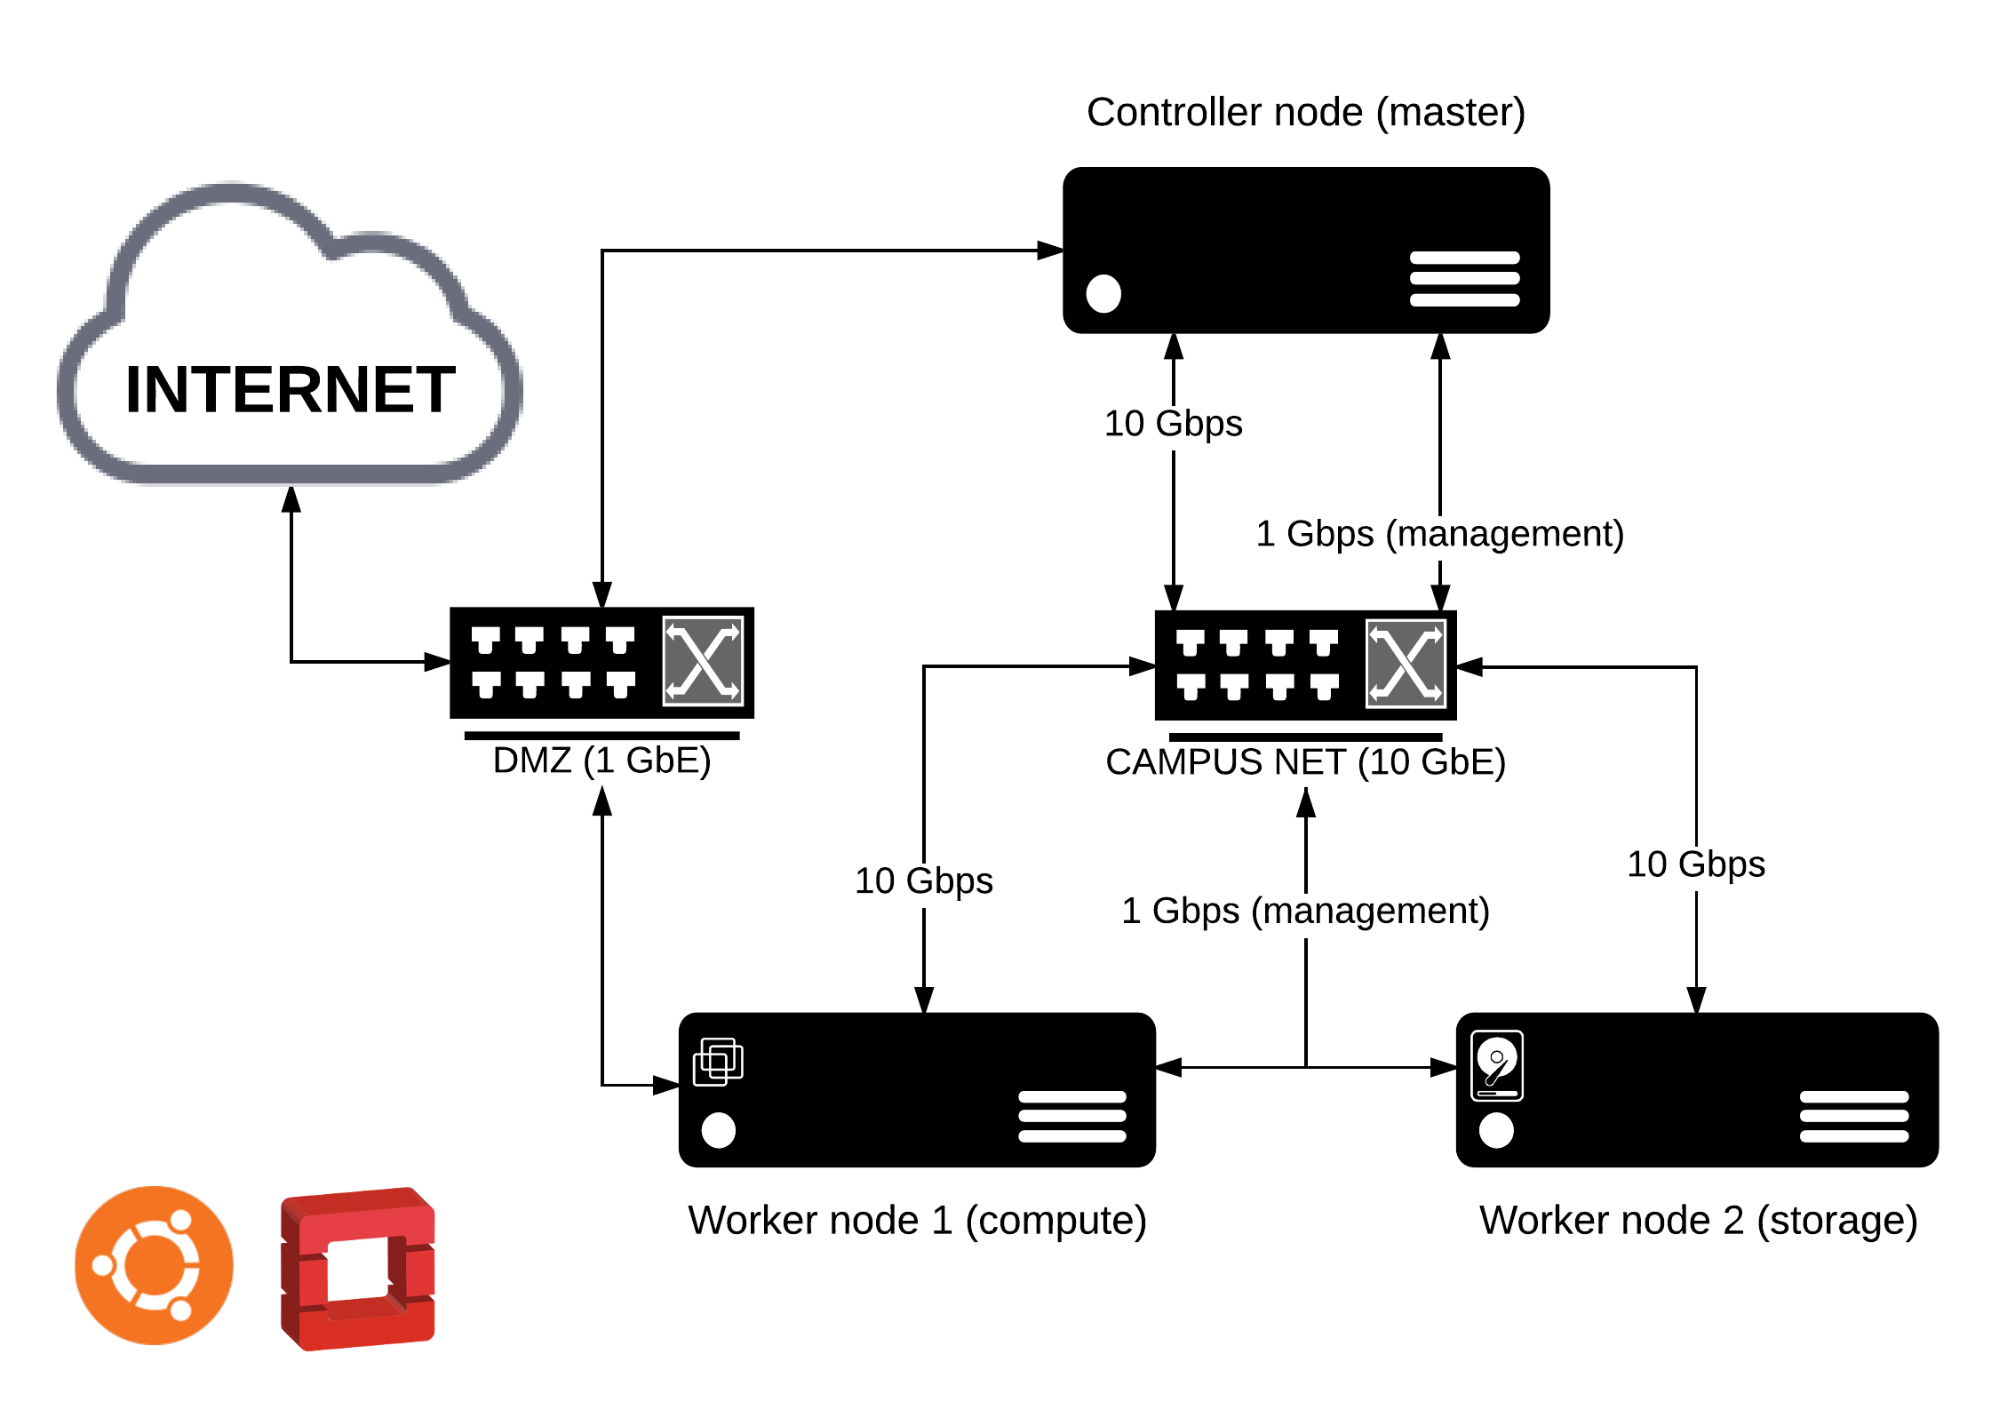
\includegraphics[width=\textwidth]{Figures/3_hardware_layout_network.png}
\decoRule
\caption[OpenStack Hardware and Network Layout]{The university-supplied internet was connected to the OpenStack controller and compute node directly. OpenStack services communicated via a 10 Gbps network and the management network was run over a more typical 1 Gbps private network.}
\label{fig:network_layout}
\end{figure}

The controller node acted as the orchestrator. Instructions are delivered to it through Nikeza and it creates virtual compute instances (virtual machines) on the first worker node while utilising storage and data that is located on the second worker node.

Each server was interconnected with 10 Gbps networking for OpenStack to communicate to all its respective services with low latency. All of the nodes were then connected to the internal network of the University of the Western Cape (UWC) through 1 Gbps interconnects to be able to interact with it and create virtual machines that use IP addresses from the UWC pool, so as to not create unnecessary security vulnerabilities by exposing the virtual machines directly to the internet. The controller and the compute worker node were connected directly to the outside internet through the DMZ on a 1 Gbps connection, in order to configure OpenStack services without IP security and port filtering rules that are in place with the standard university network.

\subsubsection{Controller Node}

The controller node aggregates and instructs services that are on other nodes. Various OpenStack services are run on this machine in order to achieve this\footnote{Installation instructions used for the OpenStack services were provided by the official documentation found at \url{https://docs.openstack.org/newton/install-guide-ubuntu/}}. The services that were on the controller node are described in Table \ref{tab:openstack_controller_services}.

\begin{longtable}[c]{@{}p{0.12\linewidth}p{0.12\linewidth}p{0.1\linewidth}p{0.55\linewidth}@{}}
\caption[OpenStack Controller Node Service List]{OpenStack services on the Controller node.}
\label{tab:openstack_controller_services}\\
\toprule
Service  & Type          & Version & Description                                                                                                                                                                                                                                                                                             \\* \midrule
\endhead
%
\bottomrule
\endfoot
%
\endlastfoot
%
Keystone & Identity      & 10.0.1  & Keystone provides an identity service to OpenStack. This provides authentication, authorisation, and cataloging of services. User accounts and roles can be created to restrict access where appropriate. Other OpenStack services also utilise it to understand which context they need to operate in. \\
Glance   & Image         & 9.1.2   & Virtual instances that are spawned on the compute node (worker node 1) need to have operating systems installed to them. Glance provides an imaging service that can store bootable images and provide them to running virtual instances on creation.                                                   \\
Nova     & Compute       & 14.0.4  & Various modules make up Nova. The controller node has Nova management services installed in order to orchestrate and manage and compute nodes that are in the OpenStack deployment.                                                                                                                     \\
Neutron  & Network       & 9.2.0   & Neutron provides OpenStack with a service that can manage virtual networks. Virtual network adapters and routes can be created to manage access to virtual instances. It provides a plugin system that allows support for various different external network configurations.                           \\
Horizon  & Dashboard     & 10.0.2  & The dashboard is an easy to use web interface to manage OpenStack as an administrator or a user.                                                                                                                                                                                                        \\
Cinder   & Block Storage & 9.1.2   & Virtual instances require disk storage to place files for operating system deployment and operation. Cinder provides block storage from any nodes running the necessary services to the virtual instances.                                                                                              \\
Swift    & Object Store  & 10.1    & Swift is an object store service that works within the OpenStack context. It is useful for storing large unstructured data. A proxy service for managing requests for data and user authentication to the storage nodes.                                                                                \\* \bottomrule
\end{longtable}

\subsubsection{Worker Node 1 (Compute)}

The first worker node was designated as the server that will handle the execution of virtual and containerised environments. This server will make use of the services available through the second worker node as well as the controller node and it is managed through the controller node. The services that are on the first worker node are described in Table \ref{tab:openstack_worker1_services}.

% Please add the following required packages to your document preamble:
% \usepackage{booktabs}
% \usepackage{longtable}
% Note: It may be necessary to compile the document several times to get a multi-page table to line up properly
\begin{longtable}[c]{@{}p{0.12\linewidth}p{0.12\linewidth}p{0.1\linewidth}p{0.55\linewidth}@{}}
\caption[OpenStack Compute Node Service List]{OpenStack services running on the Compute node.}
\label{tab:openstack_worker1_services}\\
\toprule
Service & Type    & Version & Description                                                                                                                                                                                                               
 \\* \midrule
\endhead
%
Nova    & Compute & 14.0.4  & The Nova services that runs on the compute node is comprised of a group of modules that allow for the execution of virtual machines under a pre-decided hypervisor. Since the hardware this project runs on supports hardware acceleration, the KVM hypervisor was used.                                                                                           \\
Neutron & Network & 9.2.0   & The Neutron services that run on the compute node allow for connectivity and routing from and to virtual machine instances. \\*
\bottomrule
\end{longtable}

\subsubsection{Worker Node 2 (Storage)}

The second worker node was dedicated as the storage node. This node provides block storage to all virtual instances created by the compute node, as well as the object store services which allow the storage and retrieval of data. The services running on the second worker node are described in Table \ref{tab:openstack_worker2_services}.

\begin{longtable}[c]{@{}p{0.12\linewidth}p{0.12\linewidth}p{0.1\linewidth}p{0.55\linewidth}@{}}
\caption[OpenStack Storage Node Service List]{OpenStack services running on the Storage node.}
\label{tab:openstack_worker2_services}\\
\toprule
Service & Type          & Version & Description                                                                                                                                                                                                              \\* \midrule
\endhead
%
Cinder  & Block Storage & 9.1.2   & The Cinder service on the storage node makes use of the LVM driver in order to provision physical storage that exists on it for virtual machine instances to use via iSCSI transport.               \\
Swift   & Object Store  & 10.1    & The Neutron services that run on the compute node allow for connectivity and routing from and to virtual machine instances. \\* \bottomrule
\end{longtable}

\subsection{Software}

The Python Flask micro-framework was used to rapidly create and deploy the various stages of this application.

\subsubsection{Project Breakdown}

Scheme \ref{sch:dir_tree} provides a full overview of the layout of the project on the filesystem. Where applicable, an asterisk was used in order to demonstrate that there are files in a directory that are unimportant to the operation of the software program, such as layout files.

\begin{scheme}[ht!]
% \renewcommand*\DTstylecomment{\rmfamily\color{green}\textsc}
% \renewcommand*\DTstyle{\ttfamily\textcolor{red}}
\centering
\scalebox{0.7}{\begin{minipage}{\textwidth}
\dirtree{%
.1 /.
.2 Nikeza.py\DTcomment{The main Flask application definition.}.
.2 operations\DTcomment{Directory for operational scripts.}.
.3 cloud-init.yml\DTcomment{Common cloud-init commands for VMs.}.
.2 operations.py\DTcomment{The bulk of the operational functions for working.}.
.2 parser.py\DTcomment{Parsing configuration file.}.
.2 plugins\DTcomment{Directory for plugin system.}.
.3 backend\DTcomment{Backend cloud-engine plugins.}.
.4 openstack\_bash.py\DTcomment{Plugin file to operate OpenStack with Bash.}.
.3 storage\DTcomment{Storage backend plugin.}.
.4 swift.py\DTcomment{Plugin file to operate with Swift storage.}.
.2 static\DTcomment{Directory for static media used to render frontend.}.
.3 custom.js\DTcomment{Custom JavaScript for Nikeza frontend.}.
.3 fonts\DTcomment{Fonts for Nikeza frontend.}.
.4 *\DTcomment{Various fonts.}.
.3 images\DTcomment{Images for Nikeza frontend.}.
.4 *\DTcomment{Various images.}.
.3 jstree\DTcomment{jsTree plugin for tree-view data selection.\footnotemark[\the\numexpr\value{footnote}+1]}.
.4 *\DTcomment{Various plugin files.}.
.3 materialize\DTcomment{A CSS and Javascript framework for web.\footnotemark[\the\numexpr\value{footnote}+2]}.
.4 *\DTcomment{Various framework files.}.
.3 style.css\DTcomment{Custom CSS stylesheet for frontend.}.
.2 templates\DTcomment{Directory for frontend templates.}.
.3 index.html\DTcomment{Main page for frontend.}.
.3 main.html\DTcomment{Common code shared between template files.}.
.3 new.html\DTcomment{Page for creating new job.}.
.3 queue.html\DTcomment{Page to view existing jobs.}.
.2 vars.conf\DTcomment{Variables for Nikeza runtime.}.
}
\par\null\par
*= Various unimportant files
\end{minipage}
}
\caption[Directory Tree]{Project filesystem tree hierarchy.}
\label{sch:dir_tree}
\end{scheme}
\refstepcounter{footnote}\footnotetext{jsTree by Ivan Bozhanov, \url{http://vakata.com}}
\refstepcounter{footnote}\footnotetext{MaterializeCSS framework by Materialize, \url{http://materializecss.com}}


% \begin{figure}[ht!]
% \centering
% 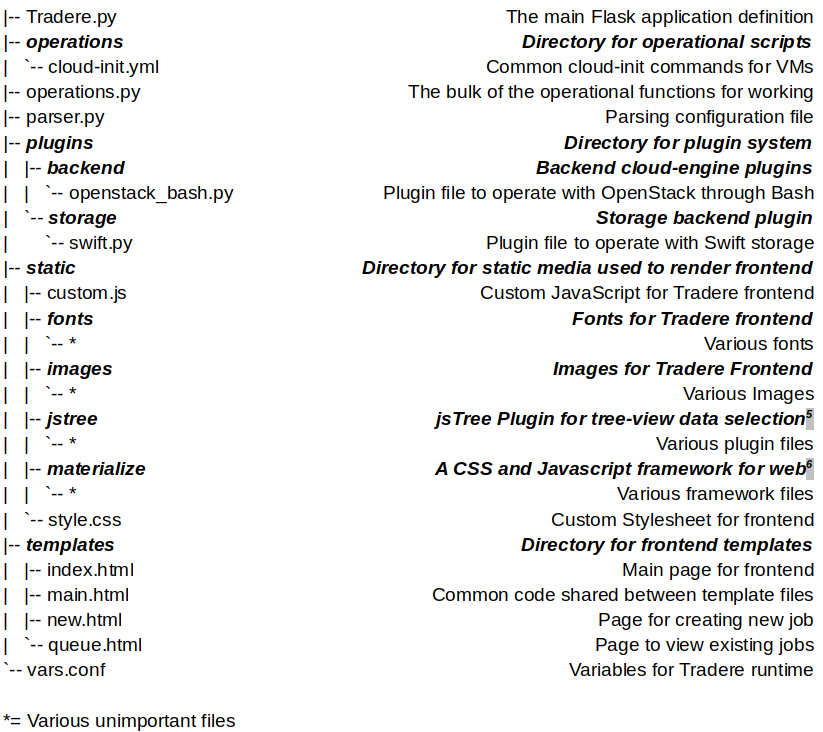
\includegraphics[width=\textwidth]{Figures/3_dir_tree.png}
% \decoRule
% \caption[Directory Tree]{Project filesystem tree hierarchy.}
% \label{fig:dir_tree}
% \end{figure}

\subsubsection{Module Dependencies}

Figure \ref{fig:module_deps} gives a visual representation of the interaction of modules and dependencies between them in the project.

\begin{figure}[ht!]
\centering
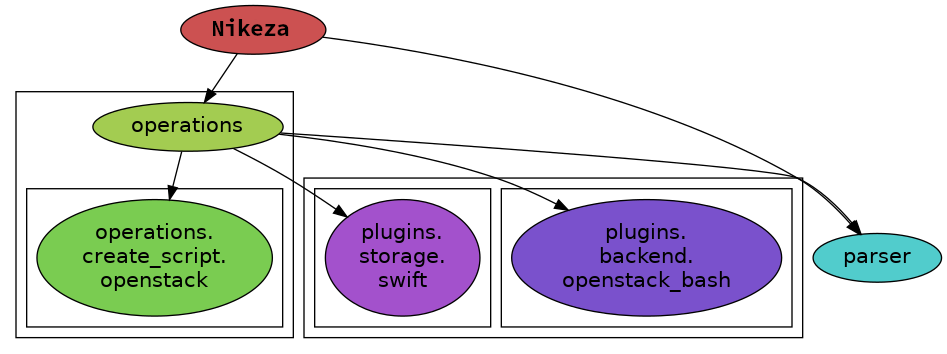
\includegraphics[width=\textwidth]{Figures/3_module_deps_new.png}
\decoRule
\caption[Nikeza Software Module Dependencies]{This figure shows the module dependencies diagram in the context of the Nikeza software.}
\label{fig:module_deps}
\end{figure}

Plugins are used with the Nikeza system in order to allow functionality with different backend cloud systems and storage services. The way this is achieved is to have a file called "vars.conf" which contains all the configuration variables for runtime. The configuration parameters are detailed in scheme \ref{sch:system_params}.

\begin{scheme}[ht!]
\makebox[\textwidth]{\fbox{%
\centering
\begin{minipage}{0.975\textwidth}
\textbf{[GENERAL]\dotfill {\small Contains variables for general configuration.}}\\
sysname=SANBI\dotfill    {\small The name of the organisation running the software}.
\par\null\par
\textbf{[BACKEND]\dotfill    {\small Contains variables for the cloud system.}}\\
platform\_name=OpenStack\dotfill    {\small The name of the backend system.} \\
platform\_file=openstack\_bash.py\dotfill    {\small The name of the plugin file for the system.} \\
platform\_image=openstack-icon.png\dotfill    {\small The name of an icon file for the system.} \\
\par\null\par
\textbf{[SYSTEM]\dotfill    {\small Contains variables for the storage system.}}\\
storage\_backend=swift.py\dotfill   {\small The name of the plugin file for the storage system.}\\
storage\_url=http://controller.cluster\dotfill    {\small The URL to access the storage with.}\\
storage\_port=8080\dotfill    {\small The port to accompany the URL.}\\
\par\null\par
\textbf{[OPERATIONS]\dotfill    {\small Contains variables for virtual machine operation.}}\\
ops\_cloudinit=cloud-init.yml\dotfill    {\small The name of the cloud-init bootstrap script.}\\
ops\_postscript=post-instance.sh\dotfill    {\small The name of the script which executes in VM.}\\
\end{minipage}
}}
\caption[System Parameters]{Global configuration file details.}
\label{sch:system_params}
\end{scheme}

The plugin files themselves are defined with a common set of classes and methods so that the operational script can successfully create instances and call methods as expected. This applies to both the cloud backend plugin and the storage system plugin.

\subsubsection{Web Rendering}

The main application file, "Nikeza.py", is used to start the Flask server, handle connections and sessions, and render the web pages. When a user navigates to one of the endpoints defined by "Nikeza.py", logic is applied to that connection and the appropriate web template is built and served to the user. This script makes use of the "operations.py" script, which handles all the backend service and platform interaction.

\subsubsection{Main Operations}

The script named "operations.py" contains all of the operations that are required for interacting with the backend environment and storage. The specifics of the interactions are detailed in the following two sections.

This file will parse the "vars.conf" file and collect all the information necessary to the application's run. It then pulls in the cloud and storage environment files as dependencies and uses their methods in order to provide the application with responses from the respective environments.

\subsubsection{Cloud Backend}

The "operations.py" script has a variable named "plugin". This variable is used to load the backend plugin file indicated by the "platform\_file" configuration line in the "vars.conf" file. This contains all the interaction commands and definitions for the cloud or appropriate backend environment that is in place. 

The file specified by "platform\_file" contains a set of common methods that can be called by the "operations.py" file. That is to say, the file specified by "platform\_file" behaves as the skeleton, or abstraction, of the backend for Nikeza. The common methods have to have a constant naming scheme between any files written for "platform\_file". These methods will have specific logic for starting virtual environments, listing running virtual machines, stopping virtual machines and retrieving IP addresses of virtual machines.

\subsubsection{Storage Backend}

Similarly to how the cloud backend is handled, the "operations.py" script contains a variable named "storage", which is used to load the storage plugin specified by the "storage\_backend" line of "vars.conf". This contains all the interaction commands and definitions for the object storage environment being used.

As with the cloud backend, the file specified by "storage\_backend" contains a set of common methods for interacting with the storage environment. This also abstracts the storage environment and allows a specific environment to be swapped out, as long as the new file is also using the same names. The methods in this file include getting the overview of the object storage contents, traversal of directories on the object store, getting object IDs and getting URLs that link to the objects in order to pull them into the virtual machines.

\subsubsection{Workflow Language}

The Common Workflow Language (CWL) specification was chosen to be used in the proof-of-concept system. This is a simple-to-learn and write language specification for researchers to wrap their pipeline into a single flowing set of reproducible instructions. The workflow language or tool chosen for the project is not critically important, as ideally many different types would be supported. For the purposes of this project, CWL is appropriate to test with due to it having various sample workflows to test.

CWL affords various executors, which are tools that parse and execute the specification. These executors offer all sorts of different functionality and targets, such as the Toil executor which can execute CWL workflows against cloud environments such as Amazon AWS. The CWL group also provides a reference executor which implements the basic functionality that a CWL executor should possess. This was deemed to be the simplest tool to use to answer the project aims posed in Chapter \ref{Chapter1}.

\subsubsection{Container System}

Docker was chosen as the container engine due to its large selection of container images available on its public repository, Docker Hub/Store, as well as it having the largest community involvement and support. The only other container engine that was considered was Singularity, due to its more research-driven focus. Singularity also allows containers to execute in a non-root environment, meaning potentially fewer complications in terms of security. 

However, due to the fact that a virtual machine is created for the researcher's execution environment and only the data that the researcher will use with the containerised tools is pulled into the said virtual machine, it was decided that Docker will be suitable. Any security risk that is presented by Docker is negated by the extra hypervisor security layer, as well as the fact that the potential attacker would already have access to the data pulled into the virtual environment even if it was through Singularity. The project was already well underway before Singularity was noticed.

There are various container orchestration systems, such as Docker Swarm\footnote{\url{https://docs.docker.com/engine/swarm/}}, Kubernetes\footnote{\url{https://kubernetes.io/}}, Red Hat OpenShift\footnote{\url{https://www.openshift.com/}} and Apache Mesos\footnote{\url{https://mesos.apache.org/}}. All of these serve to provide scheduling for multiple container instances to work together, have complex networking and communicate with shared storage together, which in turn allows them to perform more complex workloads. Originally, OpenStack's "Magnum" API extension\footnote{\url{https://wiki.openstack.org/wiki/Magnum}} was considered to be used as the core for Nikeza on OpenStack. This would have provided Nikeza native use of either Docker Swarm or Kubernetes on top of OpenStack, but it proved to be too time-consuming to implement due to the immaturity of the "Magnum" project at the time.

\section{Frontend}

The frontend part of the system is the section that the end user, or researcher, deals with directly when engaging with the project. This is the visual representation that is exposed to them. This is provided through a website that they interact with.

With reference to the above project breakdown scheme \ref{sch:dir_tree}, the "static" and "template" directories belong to the frontend part of the system. The "template" directory contains the template HTML documents that are rendered through the backend when the user requests an appropriate page. The "static" directory contains all the assets used to provide features and visuals to the user.

\section{Tools}

I would like to acknowledge that the following tools were utilised in order to complete the software project:

\begin{itemize}
    \item JetBrains PyCharm\footnote{\url{https://www.jetbrains.com/pycharm/}} - A Python Integrated Development Environment (IDE).
    \item GitHub Atom\footnote{\url{https://atom.io/}} - An Electron based hackable text editor.
    \item GitHub\footnote{\url{https://github.com/}} - A free online Git repository for source control.
    \item Pydepgraph\footnote{\url{https://github.com/stefano-maggiolo/pydepgraph}} - A tool to generate module dependency graphs for Python scripts.
\end{itemize}
% Chapter 1

\chapter{Evaluation and Comparison} % Main chapter title

\label{Chapter4} % For referencing the chapter elsewhere, use \ref{Chapter1} 

%----------------------------------------------------------------------------------------

% % Define some commands to keep the formatting separated from the content 
% \newcommand{\keyword}[1]{\textbf{#1}}
% \newcommand{\tabhead}[1]{\textbf{#1}}
% \newcommand{\code}[1]{\texttt{#1}}
% \newcommand{\file}[1]{\texttt{\bfseries#1}}
% \newcommand{\option}[1]{\texttt{\itshape#1}}

%----------------------------------------------------------------------------------------

With reference to the three research questions posed in Chapter \ref{Chapter1}, this project aims to provide researchers with a simple to use and non-technical platform with which to move workflows and research environments to where the data they intend to process is located, through the use of cloud and container technology. Nikeza aims to act as a middleman to facilitate the specification of research environments for workflows and allow the cloud environment to execute the researchers' pipeline without manual intervention. 

Nikeza needs to be compared to an alternative that is currently being used to process remote data. As mentioned in the Local Approaches subsection of the Related Work chapter, SANBI utilises remote processing locations to do some analyses already. One of the popular choices is using a cloud environment, Amazon Elastic Compute Cloud (EC\textsuperscript{2}) to be specific. Due to this, the cloud environment used to compare the process of running a workflow with Nikeza will be Amazon's Web Services. The following section will detail the comparison of executing an identical workflow remotely on Amazon EC\textsuperscript{2}, which is through use of the US-east-2 (Ohio) data center and OpenStack, which is running in a lab environment set up by the University of the Western Cape Internet Communication Services department, with Nikeza running on top of it.

It is important to clarify that the comparison between these two systems should not be seen as a comparison between OpenStack and Amazon Web Services. Rather, it is a comparison between using a cloud environment directly to execute a scientific workflow and utilizing tools or services that can automate large parts of the processes of readying the environment for said workflow execution.

The evaluation here forth will assume that the Nikeza system is already installed and made available to the user, as the installation and maintenance of the actual software system is not part of the point that this thesis paper sets out to demonstrate, but rather the use of said system.

\section{Outline}

\subsection{Task}

The task for each system is to execute a Fastqc\footnote{Fastqc is a tool which provides simple quality control checking for raw sequence data.} workflow written in the Common Workflow Language, which takes advantages of tools packages into Docker containers. The full execution command is shown in Listing \ref{lst:cwl-Fastqc}.

\begin{lstlisting}[language=bash,caption={The command specified to execute the Fastqc workflow.}\label{lst:cwl-Fastqc}]
cwl-runner fastqc.cwl --INPUT SRR5439551.fastq --nofilter --nogroup --quiet
\end{lstlisting}

The CWL workflow simply specifies that the Fastqc tool, packaged in the \url{quay.io/ncigdc} Docker image, should be run with the following arguments:

\begin{itemize}
    \item \texttt{-{}-}INPUT SRR5439551.fastq
    \begin{itemize}
        \item The input data to use, SRR5439551.fastq in this case.
    \end{itemize}
    \item \texttt{-{}-}nofilter
    \begin{itemize}
        \item Retains all reads in the output report.
    \end{itemize}
    \item \texttt{-{}-}nogroup 
    \begin{itemize}
        \item Disable grouping of bases for reads >50bp in order to show data for every base in the read.
    \end{itemize}
    \item \texttt{-{}-}quiet 
    \begin{itemize}
        \item Reduce output from the Fastqc program during execution.
    \end{itemize}
\end{itemize}

The actual workflow being used in this test is not of any real importance. The goal was to generate a result (the output data of a workflow) from an arbitrary workflow in order to prove whether Nikeza would work or not. The aforementioned workflow provided this result, by generating a small report of the data set. The task is not to determine whether workflow languages output reproducible results.

There were a number of assumptions made about the testing environments before the tests are performed. This is detailed in table \ref{tab:assumptions}.

\begin{table}[ht!]
\centering
\caption[Cloud Environment Assumptions]{Assumptions of the testing environments for OpenStack with Nikeza and AWS platforms.}
\label{tab:assumptions}
\resizebox{\textwidth}{!}{%
\begin{tabular}{p{0.5\linewidth}p{0.5\linewidth}}
\toprule
OpenStack                                                                                         & Amazon AWS                                                                                            \\ \midrule
A user account with limited standard privileges is created for the test.                          & A user account with standard privileges is created for the test.                               \\ \midrule
A Swift container is created for the test data-set to be stored on.                               & A Simple Storage Service (S3) "bucket" is created for the test data-set to be stored on.       \\\midrule
A Swift container is created for the result data to be stored on after the analysis is completed. & An S3 "bucket" is created for the result data to be stored on after the analysis is completed. \\\midrule
Both containers are made available to the test user.                                              & Both S3 "buckets" are made available to the test user.                                         \\\midrule
Test user virtual machines are allowed to access the internet.                                    & Test user virtual machines are allowed to access the internet.    
\\ \bottomrule
\end{tabular}%
}
\end{table}

\subsection{Data set}

For the testing, the so-called "Genome In A Bottle" data set was used. This data set includes reads from NA12878 and is a very well-studied and classified \parencite{paajanen2017critical}. It was chosen due to it being a manageable and relatively small set of data in order for testing and iteration on the project. 

As mentioned with the previous section, the goal is only to perform some arbitrary task and to then compare the work required to set up the analysis environment manually against the work required to use the proposed solution. As such, only the above data set was chosen to test the methodology for this project. The result of the processing on this data set will be different for different workflows, but each workflow should output reproducible results given the nature of workflow languages.

\subsection{Metrics}

\subsubsection{Number of actions for the user to perform in order to set up the workflow environment.}
The working environment for the workflow includes preparing the computer system that will be running the analysis. The operating system needs to be installed, software dependencies need to be installed on top of that operating system and data needs to be made available from the data storage of the remote environment into the working environment.

\subsubsection{Number of actions for the user to perform in order to retrieve the data from the remote environment into the workflow environment.}
Data movement still occurs in some capacity. While the data is present at the remote site, it is stored in an object store. The data needs to be copied from the object store into the computing system that is to be used for the analysis.

\subsubsection{Number of actions for the user to perform in order to execute the workflow.}
The number of actions that need to be performed in order to start and complete the analysis of the selected data.

\subsubsection{Number of actions for the user to perform in order to retrieve the processed data.}
Once the analysis is complete the data needs to be made available to be retrieved by the person who intends to use it.

\section{Results}
This section will detail the process of testing and the results of these tests. It showcases the technical steps involved in both systems, Amazon AWS and OpenStack with Nikeza, to provide perspective on how complex and time consuming using cloud environments directly can be. This is especially important in cases where researchers are not technically proficient or in an environment where the technical expertise is not available.

The "Genome in a Bottle" data set was processed with a simple Fastqc workflow using both the OpenStack with Nikeza system as well as the Amazon AWS platform. 

\subsection{Amazon AWS}

\subsubsection{Pre-work}

Two S3 buckets were created on the SANBI Amazon AWS account:

\begin{itemize}
    \item eugene.masters.data; the container that would host the data set as if it were already present on the remote system. This bucket was created on the U.S. East (Ohio) data center (Figure \ref{fig:s3_buckets}).
    \item eugene.masters.result; the container that would host the results of the researcher workflow on the remote system. This bucket was created on the U.S. East (Ohio) data center (Figure \ref{fig:s3_buckets}).
\end{itemize}

\begin{figure}[h!]
\centering
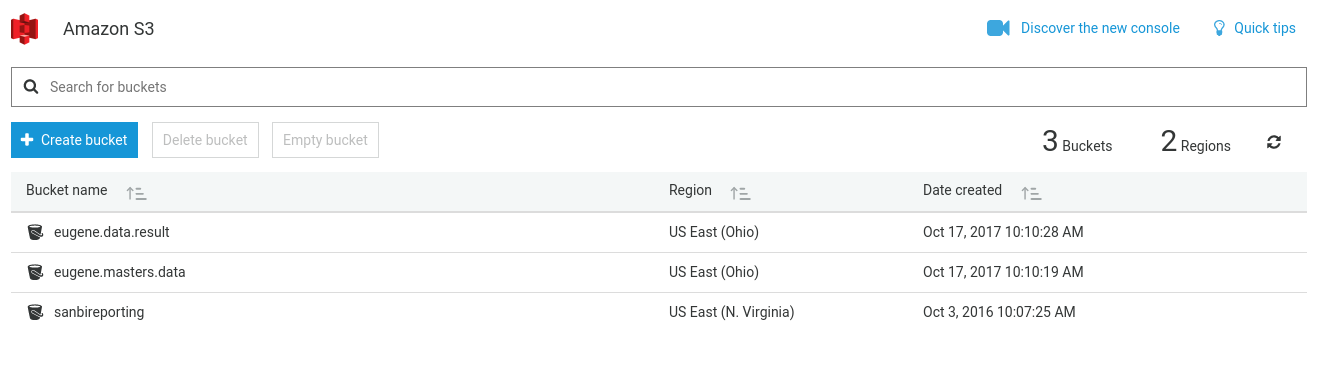
\includegraphics[width=\textwidth]{Figures/4_s3_buckets.png}
\decoRule
\caption[AWS S3 Buckets for Testing]{This figure shows the S3 buckets created for the SANBI workspace on Amazon AWS.}
\label{fig:s3_buckets}
\end{figure}

The data set (SRR5439551.fastq) was first uploaded to the eugene.masters.data bucket. This allowed it to be accessible to virtual machines that intend to use the data.

\subsubsection{Process}

The user logged into the AWS dashboard. From here, they navigate to the EC2 (Elastic Compute Cloud) dashboard. The user selected the Instances tab, followed by the "Launch Instance" button. Here, the user was presented with a list of virtual machine images to select, shown in Figure \ref{fig:aws_ami}.

\begin{figure}[h!]
\centering
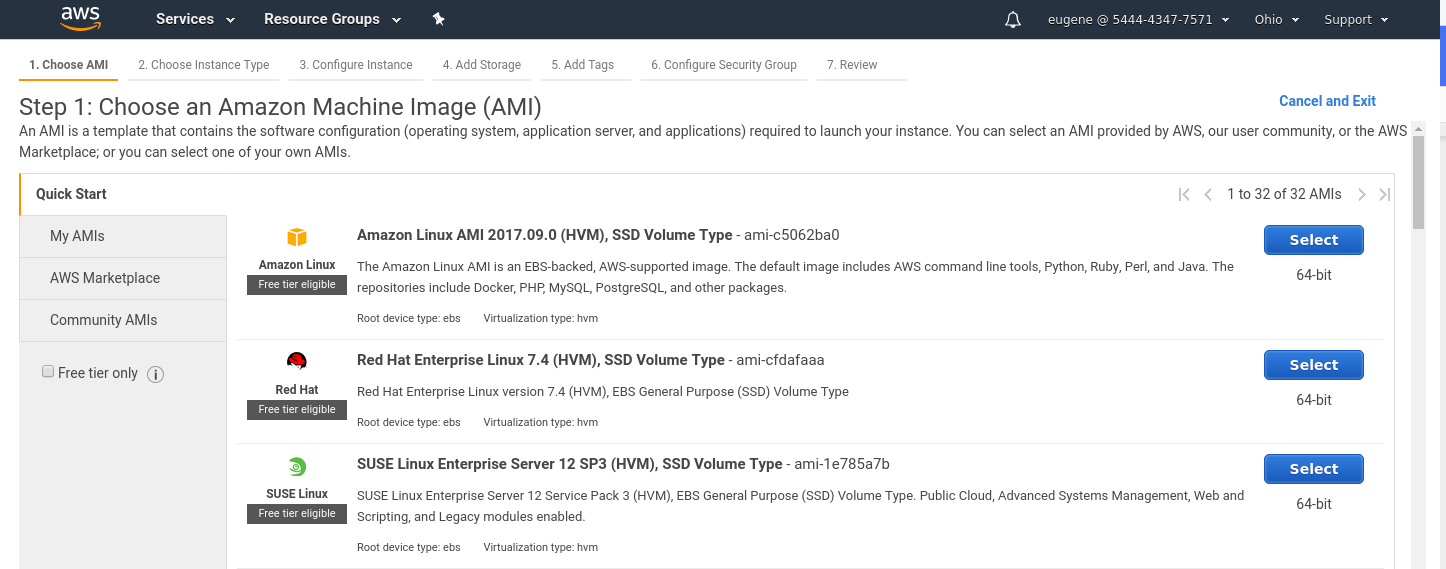
\includegraphics[width=\textwidth]{Figures/4_aws_select_instance.png}
\decoRule
\caption[List of Amazon Machine Images Available on AWS]{This figure shows the list of AMI (Amazon Machine Image) the user can choose from on the Amazon AWS web interface.}
\label{fig:aws_ami}
\end{figure}

In this case, the user would normally select whichever operating system is dictated to them or recommended by their institution. For the proof-of-concept, the Red Hat Enterprise Linux 7.4 (HVM), SSD Volume Type AMI was selected. It is also possible for the user to choose a community provided AMI here, which may include support for certain of the dependencies mentioned below out-of-the-box, however, it was not chosen in this instance due to it not being a big enough difference to the number of steps the user must take.

The next step involved selecting the instance type, which determines the hardware resource availability that is granted to the virtual instance. This is also generally dictated to the user by their institution. For proof-of-concept purposes, the General Purpose t2.micro instance was chosen. This instance type has 1 virtual CPU core and 1GB of memory available to it. This would change depending on the type of work that the user is expecting to run. The user selected the "Review and Launch" button. From the review screen, the "Launch" button was pressed and the user was presented with a screen that asked which key-pair to use for secure remote access to the virtual machine operating system environment via SSH. A new key-pair was generated in this case called eugene.masters and it was downloaded onto the computer the test was done from, shown in Figure \ref{fig:aws_keypair}.

\begin{figure}[h!]
\centering
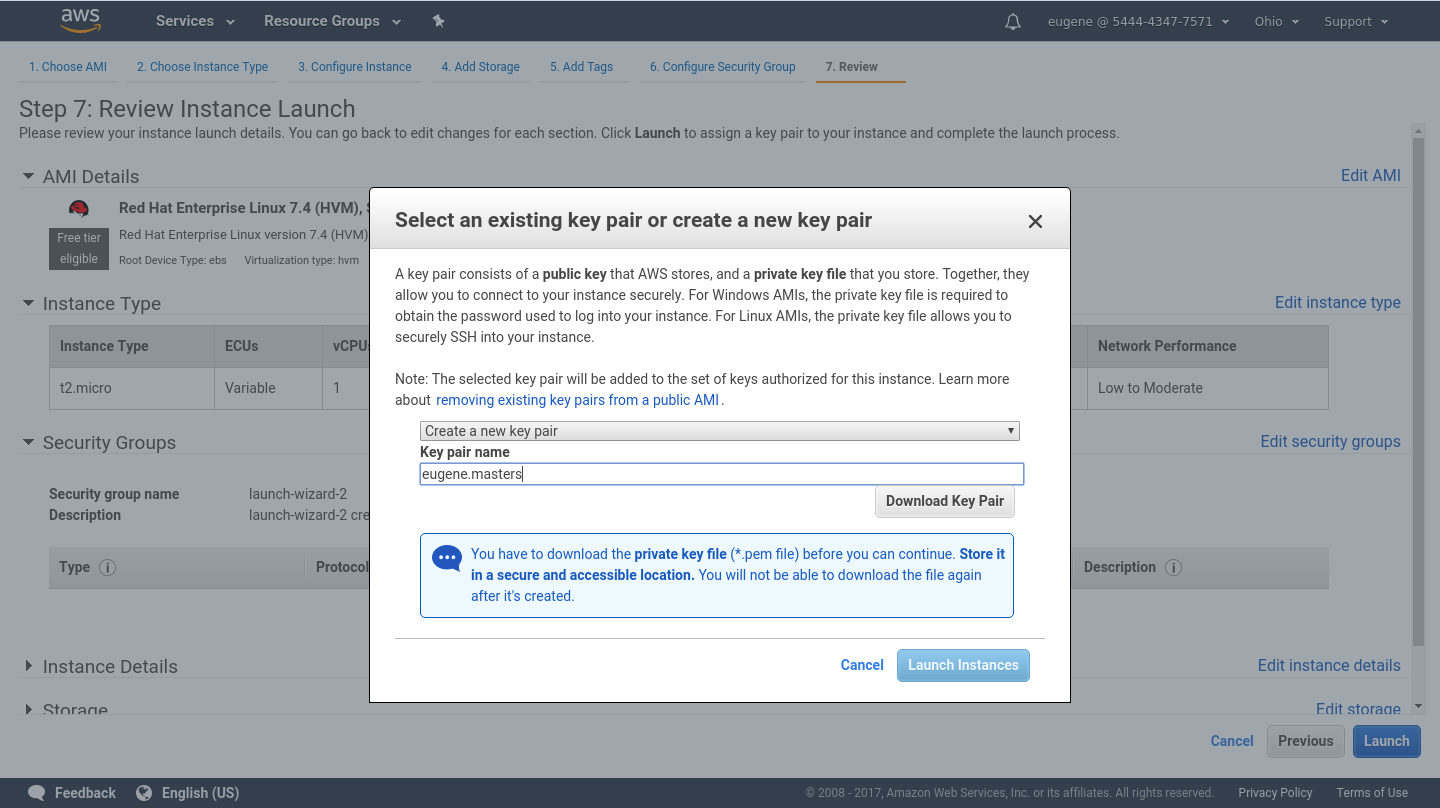
\includegraphics[width=\textwidth]{Figures/4_aws_keypair.png}
\decoRule
\caption[AWS Keypair Creation]{A demonstration of creating a key-pair to use for securely accessing the virtual instance.}
\label{fig:aws_keypair}
\end{figure}

Once the launch button was pressed by the user, they navigated back to the Instances tab in order to retrieve their IP address for accessing the virtual machine. The IP address is available from the dashboard as illustrated on the right of Figure \ref{fig:aws_instancelist}. 

\begin{figure}[h!]
\centering
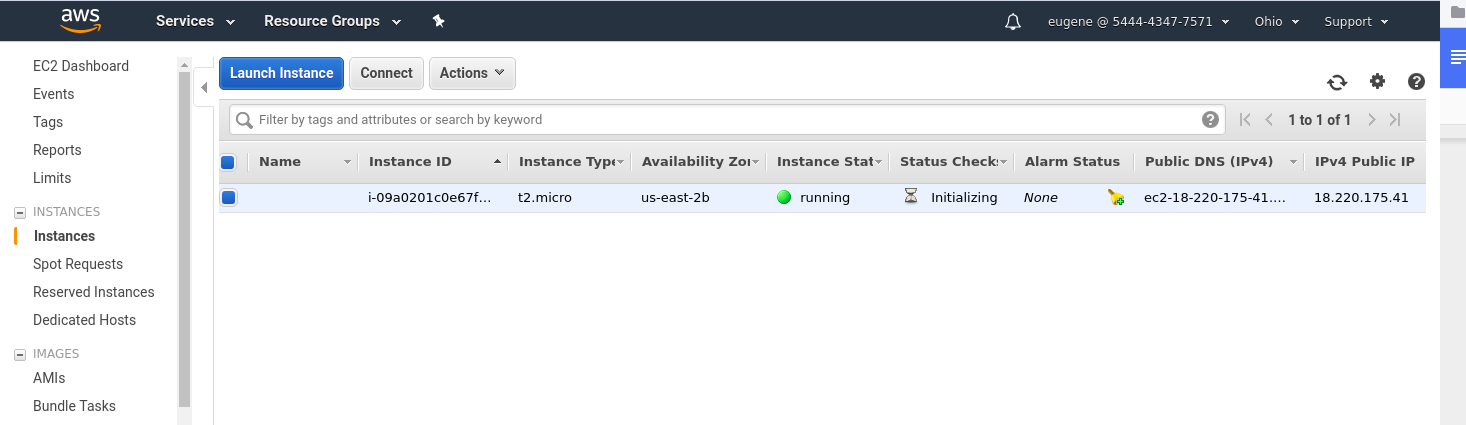
\includegraphics[width=\textwidth]{Figures/4_aws_instancelist.png}
\decoRule
\caption[AWS Instances View]{This is the Instances tab on the Amazon AWS web interface for the user, where the public IP address is retrieved.}
\label{fig:aws_instancelist}
\end{figure}

The user was required to change the permission of the key file that was downloaded from AWS when creating the instance to Unix permission set 400 if on Linux, or use an SSH client such as PuTTY on Windows. The user then created an SSH session into the virtual environment via the command shown in Listing \ref{lst:ssh}.

\begin{lstlisting}[language=bash,caption={The utilising of the key in order to access a remote terminal session in the new virtual instance.}\label{lst:ssh}]
ssh -i eugenemaster.pem ec2-user@18.220.175.41
\end{lstlisting}

Running this command provided the user with a bash terminal inside of the virtual machine hosted by Amazon.

For the user to be able to retrieve data from an S3 bucket, they needed to ensure that the tool being used to do so could authenticate the user. The user retrieved the Access Key ID associated with their account under the Users dashboard in the AWS console by selecting "Create Access Key" after which they took note of the ID and the secret key.

In order for the user to retrieve the data from the AWS S3 bucket, they were required to download it into the running instance. This was done through Amazon supplied CLI tools that were installed to the container. This step could have also been accomplished using standard Linux tools, but introduce additional complexity. First, the user navigated to the S3 dashboard in order to retrieve the endpoint and location of the data on the S3 bucket. The AWS CLI tool was installed onto the virtual instance. In order to do this, the user executed the command shown in Listing \ref{lst:aws_cli_install}.

\begin{lstlisting}[language=bash,caption={Executing the shell command to install the Amazon command-line tools for interacting with AWS.}\label{lst:aws_cli_install}]
sudo easy_install awscli
\end{lstlisting}

This installed the AWS CLI tool onto the virtual instance using the Python package manager. The Python installation method is the simplest and quickest way to get this tool running in this case. Once complete, the user configured their credentials by executing the command shown in Listing \ref{lst:aws_conf}.

\begin{lstlisting}[language=bash,caption={Setting up the initial AWS tool configuration.}\label{lst:aws_conf}]
aws configure
\end{lstlisting}

Here the user entered the Access Key ID, Secret Access Key, region that the data exists on (us-east-2 in this case) and output format, after which they executed the command in Listing \ref{lst:aws_s3_cpy}.

\begin{lstlisting}[language=bash,caption={Using the AWS tool to copy the data from the S3 bucket to the virtual instance.}\label{lst:aws_s3_cpy}]
aws s3 cp s3://<bucket name>/<file name> .
\end{lstlisting}

In this case, the bucket name was eugene.masters.data and the file name SRR5439551.fastq, which is the data that was to be processed. This command will copy the data from the cloud provider's storage to the storage that the virtual instance has access to.

Once the data was on the virtual instance, the user installed the tools necessary for executing the workflow. For the Fastqc workflow sample, this was Docker and cwl-runner. With Red Hat Enterprise Linux (RHEL), Python version 2 is shipped by default. cwl-runner requires Python version 3, however, this does not exist in the default RHEL repositories. A custom repository needed to be added in order to install cwl-runner, shown in Listing \ref{lst:aws_setup_os}.

Once completed, the other dependency for the workflow needed to be installed. Docker is also not contained in the repositories for RHEL and as a result, the steps on the Docker website were followed in order to install it: \url{https://docs.docker.com/engine/installation/linux/docker-ee/rhel/}. Once Docker was installed, the daemon process was enabled and started as shown in Listing \ref{lst:aws_docker}.

\begin{minipage}{\linewidth}
\begin{lstlisting}[language=bash,caption={The steps for adding the repository to RHEL for retrieving Python 3 and cwl-runner.}\label{lst:aws_setup_os}]
sudo rpm -ivh \ https://dl.fedoraproject.org/pub/epel/epel-release-latest-7.noarch.rpm
sudo yum -y install https://centos7.iuscommunity.org/ius-release.rpm
sudo yum -y update
sudo yum -y install python36u python36u-setuptools
sudo easy_install-3.6 cwl-runner
\end{lstlisting}
\end{minipage}

\begin{lstlisting}[language=bash,caption={Enabling and starting the docker service.}\label{lst:aws_docker}]
sudo systemctl enable docker && sudo systemctl start docker
\end{lstlisting}

It is important to note that if the user decided to download the data from the S3 bucket into the virtual machine after this step instead of doing it earlier, the user could create their own AMI "snapshot" of the virtual machine in this current state, which would make it easier to get up-and-running for a future deployment of workflows that rely on Docker and CWL. This does not translate to other cloud providers if they need to run this workflow at other sites.

Now the CWL workflow was uploaded to the instance using scp. Any other tool which allows the workflow to be moved could also have been used. 

For RHEL specifically, in order to execute the workflow the user needed to disable SELINUX on the operating system. This was done by changing the "enforcing" line to "disabled" in the file /etc/selinux/config. If this is not done, cwl-runner would not have been able to write output to the file system of the operating system and would have failed as a result. The virtual instance was rebooted for changes to take effect. Once rebooted, the user executed the workflow as shown in Listing \ref{lst:aws_cwl_exec}.

\begin{lstlisting}[language=bash,caption={Executing the workflow on RHEL with cwl-runner installed and data copied.}\label{lst:aws_cwl_exec}]
sudo cwl-runner fastqc.cwl --INPUT SRR5439551.fastq --nofilter --nogroup --quiet
\end{lstlisting}

Once the process was complete, the user received a message "Final process status is success" from the tool, after which the user was then able to retrieve the output file from the virtual machine whichever way they wish, for example downloading it through scp directly from the virtual machine or uploading it to an s3 bucket as in this case. The data was uploaded to the eugene.masters.result bucket. Once the upload succeeded, the user could navigate to the S3 dashboard, select the bucket and download the data from there as shown in Figure \ref{fig:aws_s3_result}.

\begin{figure}[h!]
\centering
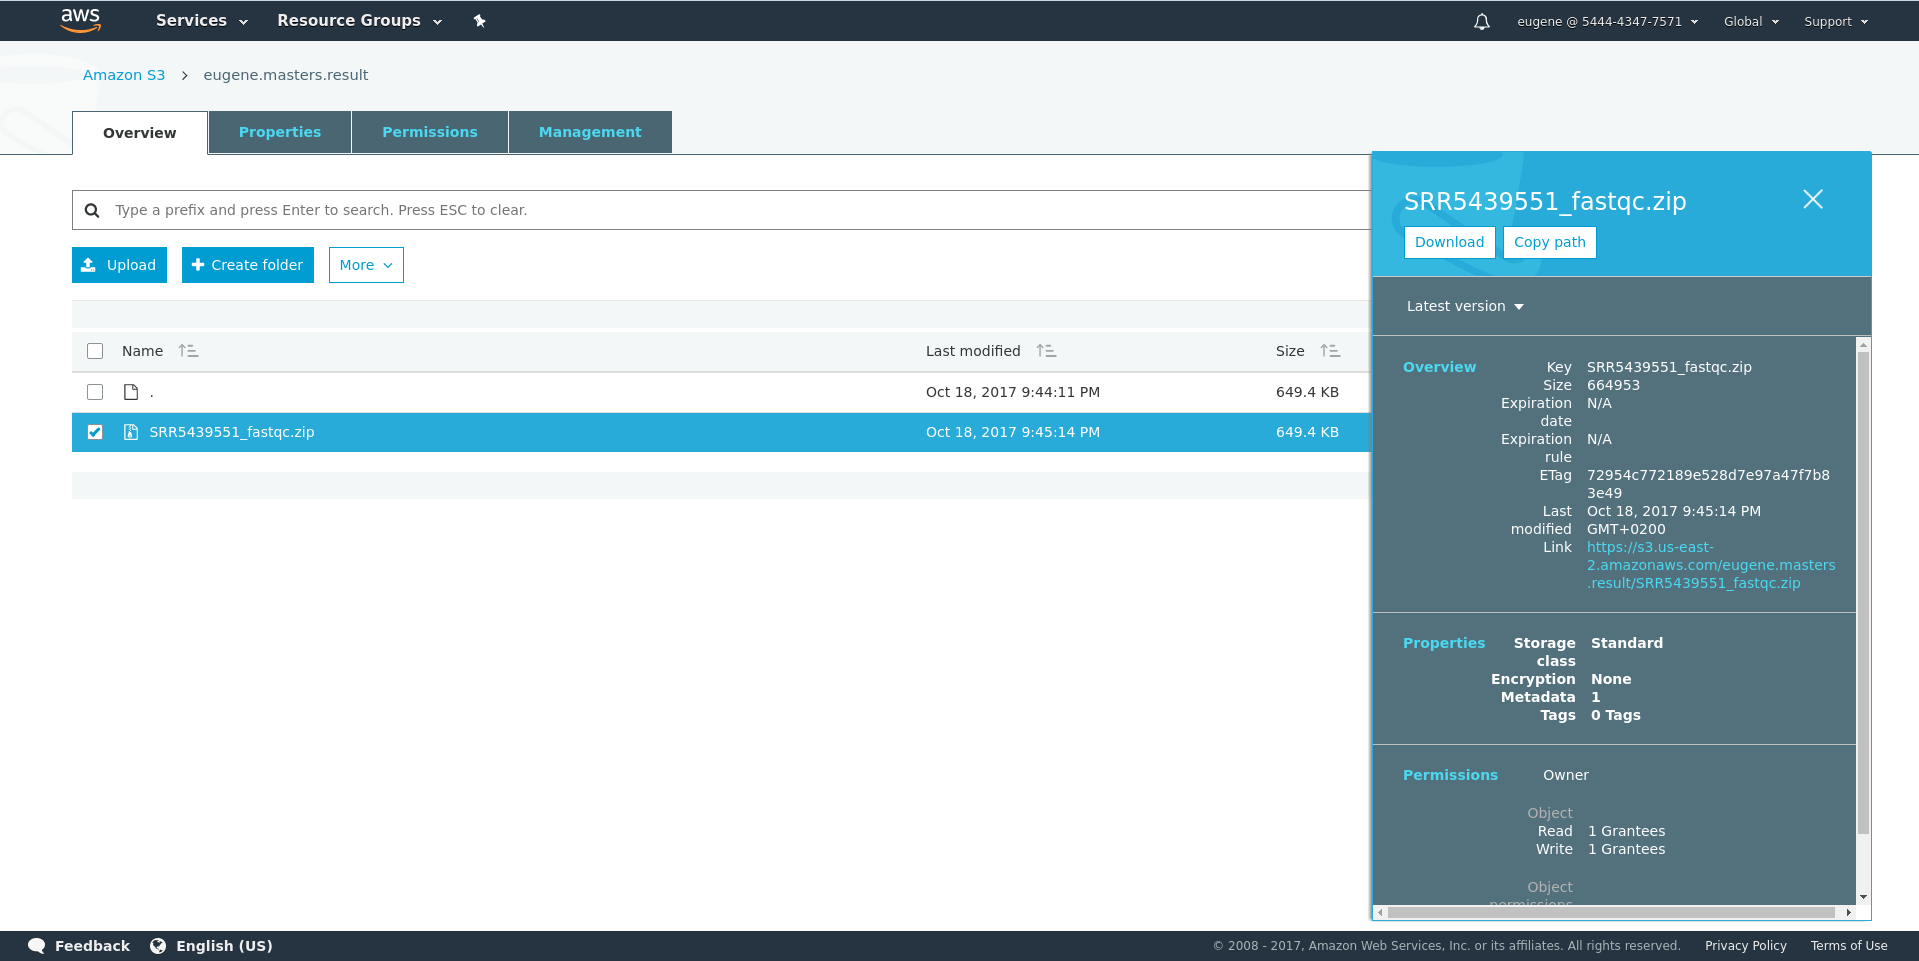
\includegraphics[width=\textwidth]{Figures/4_s3_bucket_result.png}
\decoRule
\caption[AWS S3 Bucket with Result Data]{This shows the data generated from the workflow stored in the eugene.masters.result S3 bucket.}
\label{fig:aws_s3_result}
\end{figure}

\subsection{OpenStack with Nikeza}

\subsubsection{Pre-work}

Two Swift containers were created on the OpenStack backend for the test user.

\begin{itemize}
    \item seqdata; the container that would host the data set as if it were already present on the remote system (Figure \ref{fig:swift_prep}).
    \item resultant; the container that would host the results of the researcher workflow on the remote system (Figure \ref{fig:swift_prep}).
\end{itemize}

\begin{figure}[h!]
\centering
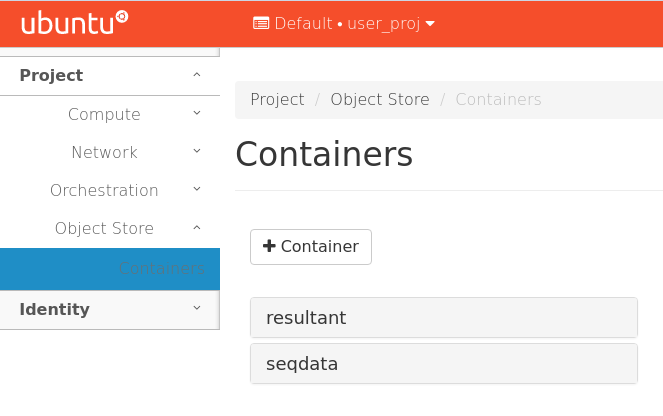
\includegraphics[width=\textwidth]{Figures/4_os_swift_prep.png}
\decoRule
\caption[OpenStack Swift Containers for Testing]{This shows the data containers created in Swift in the OpenStack system for the user.}
\label{fig:swift_prep}
\end{figure}

\subsubsection{Process}

The data set (SRR5439551.fastq) was first uploaded to the eugene.masters.data bucket. This allowed it to be accessible to virtual machines that intend to use the data.

With the Nikeza system in place, a user needs to navigate to the website that provides the Nikeza interface. Here the user was presented with a login screen on which they must enter their credentials for the cloud environment of that institution (provided to them through that institution or based on federated authentication). This screen is shown in Figure \ref{fig:os_login}.

\begin{figure}[h!]
\centering
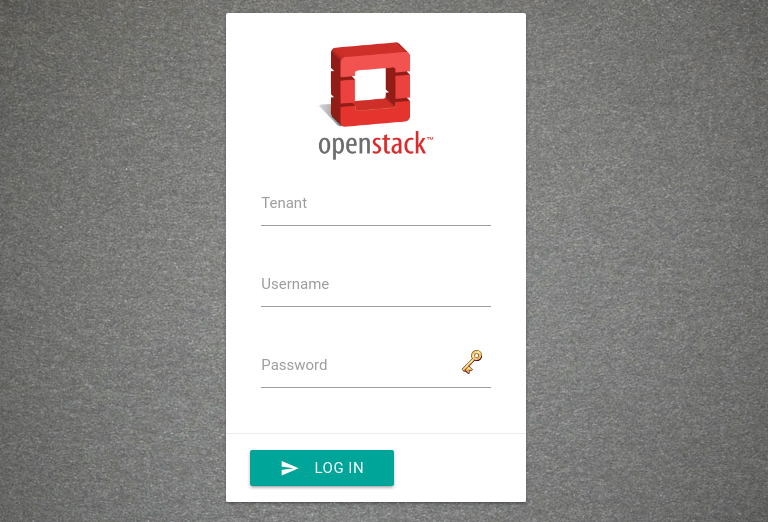
\includegraphics[width=\textwidth]{Figures/4_os_login.png}
\decoRule
\caption[Nikeza Login Screen]{This image shows the Nikeza login screen configured with OpenStack backend.}
\label{fig:os_login}
\end{figure}

Once the user was logged in, they were provided a dashboard which showed their queued and running jobs shown in Figure \ref{fig:os_queue}. There were no active jobs for the user. Two buttons below the queue are shown, one to create a new job and one to stop any selected jobs.

\begin{figure}[h!]
\centering
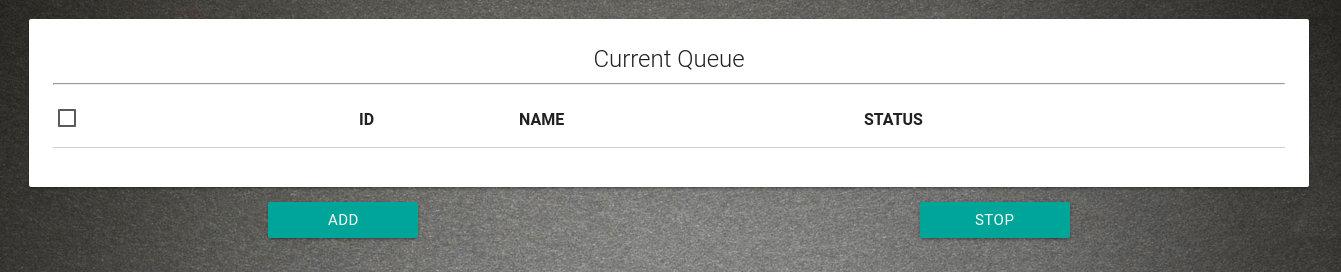
\includegraphics[width=\textwidth]{Figures/4_os_queue.png}
\decoRule
\caption[Nikeza Job Queue Page]{The Nikeza queue page with no active jobs.}
\label{fig:os_queue}
\end{figure}

The user clicked the button to create a new job. As shown in Figure 6.9, the page that they were provided with asked the user to upload the workflow file that they would have written or retrieved from another source, fastqc.cwl in this case, followed by the arguments for the workflow shown in Listing \ref{lst:os_cwl_comm}.

\begin{lstlisting}[language=bash,caption={The arguments for the workflow in question.}\label{lst:os_cwl_comm}]
--INPUT SRR5439551.fastq --nofilter --nogroup --quiet
\end{lstlisting}

The user then selected the data they wish to process from a list provided to them in the second step box, they selected the directory in the virtual machine that the data would be placed, or copied, in step 3 and where the resultant data would be created in the virtual machine in step 4 and finally which container the user wants the data to be uploaded to the cloud environments storage solution.

\begin{figure}[h!]
\centering
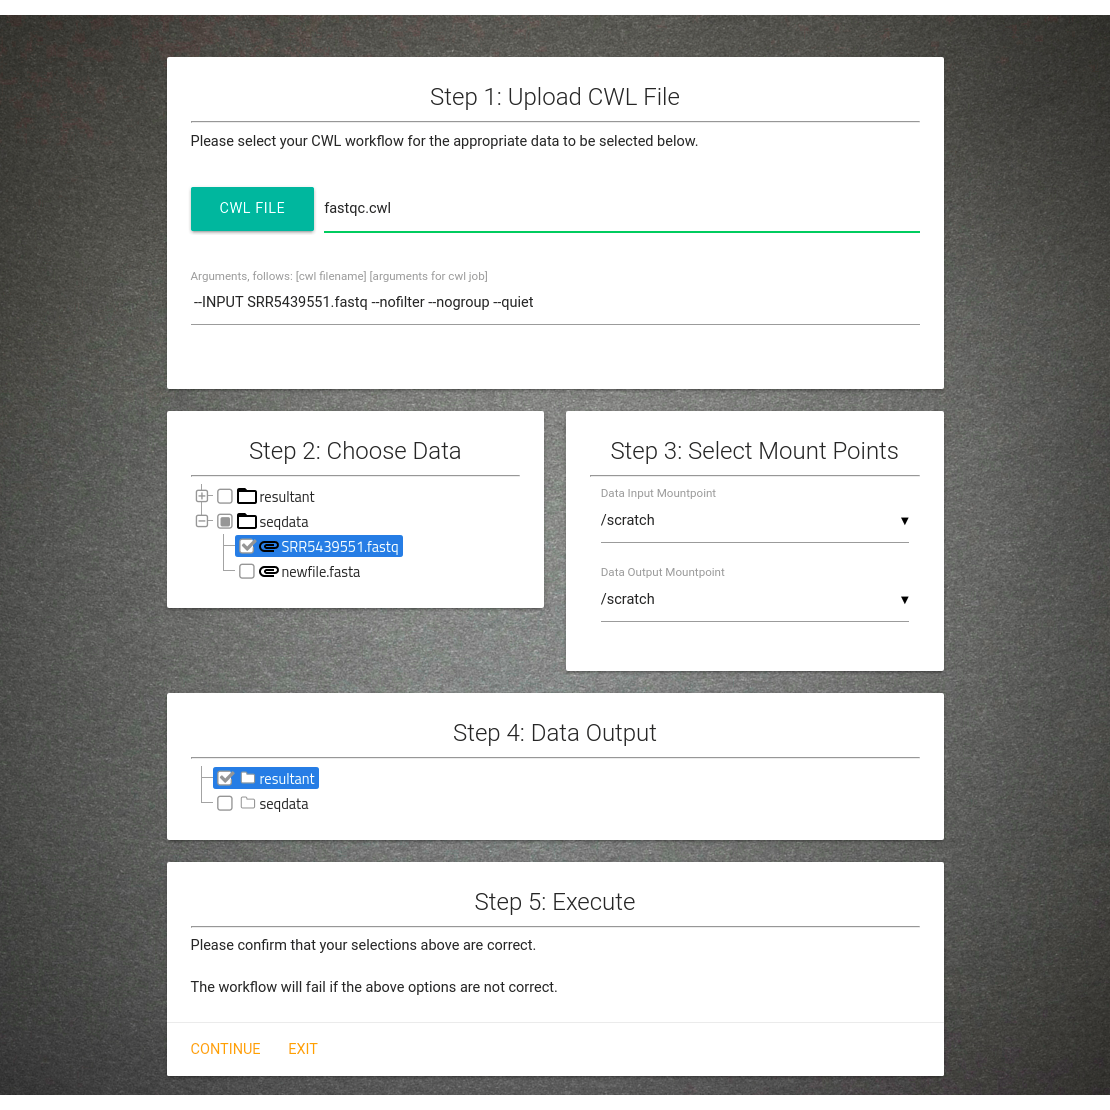
\includegraphics[width=\textwidth]{Figures/4_os_config.png}
\decoRule
\caption[Nikeza Workflow Configuration Screen]{The Nikeza workflow creation and configuration page, where the user will select the CWL file they wish to execute and the details around the workflow.}
\label{fig:os_conf}
\end{figure}

The user clicked the button to start the workflow (CONTINUE) and waited on the processing to finish. Once the workflow was completed the data was uploaded to the container specified by the user, the resultant container in this case, and the virtual machine was destroyed. The user could now fetch the data from the resultant container, shown below in Figure \ref{fig:os_result}.

\begin{figure}[h!]
\centering
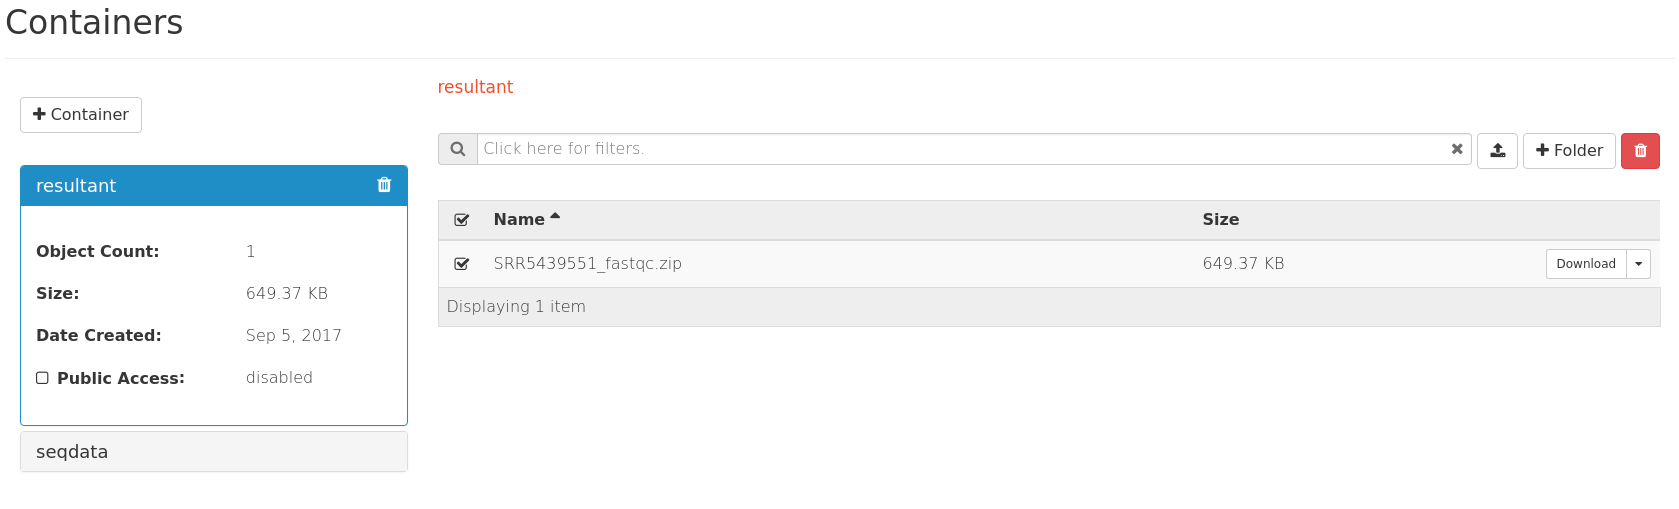
\includegraphics[width=\textwidth]{Figures/4_os_swift_result.png}
\decoRule
\caption[OpenStack Swift Container with Result Data]{This shows the data generated from the workflow stored in the resultant OpenStack container.}
\label{fig:os_result}
\end{figure}

\subsection{Summary}

It should be clear that from a user perspective, using the cloud directly involves a substantial amount of additional work than using something such as the project demonstrated in this thesis. The below sections summarise the differences (also see Table \ref{tab:comparison_overview}).

\subsubsection{Amazon AWS}
The user must navigate to the website and log in with their credentials for the cloud provider. They must then navigate to the correct tab where they can create instances (virtual machines) to run their work. Once there, they can create a virtual machine by selecting the image type that they want, followed by the instance type. If the user has already created a key pair then they may select to use that or to create a new key pair, otherwise, they will be prompted to create a key pair for the instance. Assuming no key pair was created prior to the creation of the virtual machine instance, the user must then download the newly created key pair and set the correct permission on the file. They can now log into the instance via an IP address shown to them in the instance menu on the cloud dashboard. Once inside, they can install the cloud provider tools to access the data storage, configure the tools with their account details and download the data onto the running instance. Before running the workflow, they must ensure that Docker is installed and activated and that a CWL executor is installed onto the instance. They can then safely start the workflow.

When the workflow completes, the user must upload the data from the instance to the cloud storage of the provider using the same method of retrieving the raw data. Once complete they will be able to retrieve the results from the storage page on the cloud provider dashboard. The last step for the user is to shut off the running virtual instance.

Each time that a user wants to run a workflow they will need to start a virtual machine instance. The setup of these instances can be reduced by using an available pre-built image or AMI, but setting up the AMI from the Amazon Web Service interface, retrieving the data to the virtual instance, copying the workflow scripts and executing it need to be done every time a workflow needs to be run. Additionally, modifications may potentially need to be made on images if they are to run different workflows.

\subsubsection{Nikeza}
The user must navigate to the Nikeza dashboard and log in with their provided cloud credentials. Once logged in, they can click the "Add" button on the page they are presented with. The next page presents them with a form where they can select the workflow file from their local computer, specify the arguments for the workflow and select the data they want to process. After completing the form, the user clicks the "CONTINUE" button. The workflow environment is now being prepared and the workload is being executed in the background automatically.

When the workflow completes, the user will be able to retrieve the results from the storage page on the dashboard of the cloud provider being used behind Nikeza. The virtual machine instance is shut down for the user.

This is the procedure that occurs each time a workflow needs to be executed. The interface stays much the same and the user just selects the items that they want to process and select the data that they want to process on.

\subsubsection{Overview}


% Please add the following required packages to your document preamble:
% \usepackage{booktabs}
\begin{table}[ht!]
\renewcommand\footnoterule{}
\caption[Step Differences between Nikeza and Amazon AWS]{The differences between steps needed to complete the work task using OpenStack with Nikeza and Amazon AWS.}
\label{tab:comparison_overview}
\resizebox{\textwidth}{!}{%
\begin{tabular}{p{0.7\linewidth}p{0.15\linewidth}p{0.15\linewidth}}
\toprule
                                                                                                                                   & OpenStack with Nikeza & Amazon AWS \\ \midrule
Number of actions for the user to perform in order to set up the workflow environment.                                                           & 5                     & 15\footnote{This figure could be lowered around 3 actions if the user utilized an AMI that has some of the software dependencies pre-installed.}         \\ \midrule
Number of actions for the user to perform in order to retrieve the data from the remote environment into the workflow environment. & 0                     & 4          \\ \midrule
Number of actions for the user to perform in order to execute the workflow.                                                        & 1                     & 8          \\ \midrule
Number of actions for the user to perform in order to retrieve the processed data.                                                 & 3                     & 3          \\ \midrule
TOTALS                                                                                                                             & 9                     & 30         \\ \bottomrule
\end{tabular}
}
\end{table}

\section{Discussion}

An almost identical process occurs for both systems. A virtual machine is created, software dependencies are installed, data is retrieved, processed and made available for the user to either download or use in another workflow or process. For both of the aforementioned processes, the data that was generated was identical. The difference is in the ease and speed of actually executing the workflow that the researcher desires to do on the data set. While it is true that in both cases the data does not need to be moved from the cloud environments to the researcher first in order to do the work on it, assuming that the data was uploaded beforehand, it is clear that one of the solutions is significantly more time consuming and technically involved.

The Amazon AWS, or direct cloud, approach requires a greater deal of not only technical knowledge (depending on the virtual environment that the researcher is using), but also takes significantly longer to get into a state where the researcher is able to process their workflow. This can be mitigated by the cloud environment providing pre-built virtual images (AMIs in the case of Amazon) that contain the tools that a researcher would need, but this is not common and is also not manageable given all the novel requirements that various researchers have for their workflows. Virtual images have been created on the Amazon AWS by other users and groups which contain the necessary CWL runtimes, or various other software packages as mentioned, pre-installed. This allows users to execute containerized workflows in a similar fashion to Nikeza, removing the graphical environment. The user can even run through the above-mentioned procedure and create a snapshot of the virtual environment to reuse when they wish to execute workflows in the future, saving time after the initial creation of the environment.

The Nikeza system greatly simplifies the creation and dependency management of the virtual environment for the researcher. By providing the researcher with an intuitive and simple to follow interface for uploading their workflow and selecting their data set, the researcher is able to more rapidly submit workflows to be processed. It also reduces the need for a researcher to be reliant on additional personnel such as a technical person in order to assist them with creating the environment in the first place. Nikeza's advantage is that it can encourage the deployment and development of more localised private cloud environments that can be run by institutions, potentially providing avenues for the development of skills and collaboration of different types of science. It does not only need to be constrained to private clouds and could even be applied to public cloud environments.

On the other hand, some drawbacks of this kind of approach are that much development time is necessary to turn it into a product that can actually be used in production workflows in a reliable manner. It is also potentially necessary to have some person dedicated to the maintenance of the software at the various institutions it is to be deployed. It also competes with existing workflow deployment tools which in recent times have made much progress to being simpler to use and more reliable.

OpenStack itself was not tested separately due to the fact that it is very similar to how the user would engage with AWS. OpenStack exposes a very cloud-computing like dashboard to the end user if using Horizon (the OpenStack Dashboard system) directly. Due to this, the test between directly using OpenStack and Amazon AWS would result in mostly the same steps to be taken with some minor differences in syntax.

It is important to note that this is not an extensive test. This project did not set out to compare cloud environments themselves, but rather show the usefulness of solutions that can exist to compliment these clouds for scientific use. Many solutions for executing workflows on the cloud are becoming more popular by the day. One example is the Toil executor for CWL which has implemented support for deploying workflows to public clouds from the user's desktop \parencite{vivian2017toil}, requiring some pre-setup on the user side.
 
% Chapter 1

\chapter{Summary and Future Work} % Main chapter title

\label{Chapter5} % For referencing the chapter elsewhere, use \ref{Chapter1} 

The results of this project are the groundwork for further investigation of the simplification of cloud environments for researchers. With cloud computing continuing to grow, it is possible to have these kinds of services, such as Nikeza, integrated with it directly in a more researcher focused effort. More cloud environments are being adopted as the go-to platform for delivering flexible scientific analysis. This is evident from projects such as the SADIRC being built from the ground up to support astronomy and bioinformatics workloads and the Cloud Infrastructure for Microbial Bioinformatics (CLIMB) system which a research cloud environment built to provide resources for microbial bioinformatics in the United Kingdom \parencite{connor2016climb}.

\section{Summary and Conclusions}

In light of the issues raised in Chapter \ref{Chapter1}, such as data growth becoming an increasingly difficult problem and technical skill being a requirement to use modern cloud computing environments, this project aimed to provide a solution. A proof-of-concept automation tool for researcher workflows, named Nikeza, was designed and prototyped. This tool provided a simpler and non-technical approach to utilising the cloud environment.

Deployment of Nikeza was done using a local private cloud environment built using OpenStack as a base, which allowed it to be compared in executing a research workflow against existing cloud environments of a similar nature, namely Amazon AWS, given the assumption that the data to be processed was already at the location. 

The results showed that using Amazon AWS for research purposes is very possible. However, this requires a detailed technical knowledge of how to utilise not only the Amazon provided web dashboard, but also the virtual machines created on it themselves. With the Amazon AWS test, the researcher is required to navigate through a maze of different dashboards which provide information on the different services that are on offer. They are required to create a virtual machine with a pre-built operating system image that provides them with the required base to begin, followed by the installation of their entire work environment. The researcher must also manually ensure that the data they wish to operate on is pulled into the virtual environment in some fashion. Once this is completed, the researcher may move their workflow to the platform in order to execute it and they are left to retrieve the data from the virtual machine and shut it down manually. The only way that this can be simplified for researchers is if the organisation they work for provides pre-built virtual machine images with the necessary work environment or tools installed, but this leads to issues of maintaining those and creating environments for every novel approach which is unmaintainable.

In comparison, the work done in the Nikeza project provided a simpler platform for researchers to perform remote computational work through a workflow language. More specifically, it looked at addressing the three key aims of 1) the moving of workflows to the cloud, 2) simplifying cloud environments for researchers, and 3) integrating workflow languages into the cloud.

\paragraph{Moving Workflows to the Cloud}
Workflow language specifications or tools allow researchers to define an instruction specification for the analysis. The fact that most provide ways of fetching tools from local or non-local sources means that the movement of this specification is very easy and portable. The tests conducted for this thesis show that these technologies compliment a cloud environment and promote a focus on research, rather than system preparation and allowed the size of the data that needed to be sent from the researcher to the remote environment to be relatively tiny.

\paragraph{Simplification of Cloud Environments}
The comparison between the Amazon cloud on its own and OpenStack cloud with Nikeza shows, when running the same workflow, that it is substantially easier to use Nikeza from a researcher perspective. All of the technical work is automated and abstracted for the researcher, allowing them to focus on what they want to accomplish. The researcher merely has to log in to the dashboard, upload their workflow script, provide the flags for the workflow, select the data and the placement of the data, and finally where the data is sent to upon completion. This is provided in one simple interface for the researcher and they are never expected to interact with the virtual environment at all. This proof-of-concept demonstrates the viability of creating easy-to-use interfaces to the cloud.

\paragraph{Integrating Workflow Languages into the Cloud}
The integration of workflow languages can be done in two ways. The way that this thesis project demonstrated it was to create a software platform that interacts with a cloud environment to utilise its functions on behalf of a user. This is a flexible and customisable approach. The other way is for cloud providers to treat workflow languages as a first-class citizen and offer their own workflow language integration directly into their platforms.

This project has successfully managed to answer all three posed research questions and has achieved the majority of the technical functionality requirements laid out for the system as mentioned in Chapter 4, section 4.6. The technical functionality aspect that was not reached was to create a fully modular system for ease of replacing plug-ins to support different cloud environments. This was not achieved due to time constraints and it being a greater task than originally envisioned. Currently, the application is very strongly tied with the OpenStack platform.

The Nikeza project has successfully demonstrated that researchers are able to analyse their data at the site where the data is being generated. It allows researchers to provide their own analysis environments and process data exactly the way that they expect, without having to rely on specific tools to be made available from the institution. It also shows that reproducible scientific workflows can fairly easily be used on top of cloud environments, taking advantage of efficient resource usage.

\section{Future Work}

During the completion of this thesis, the landscape for research analysis on the cloud has changed. It is important to note that there have been progressions by other projects into utilising the cloud in a way that this thesis project aimed to do. While not identical to this approach, projects such as Galaxy also serve to prove the usefulness of adapting the work onto scalable and distributed cloud environments. The South African Medical Research Council also announced the launch of the African Genome Center that will be a local sequencing facility. The architecture outlined in this thesis would be well suited to a sequencing facility such as the African Genome Center.

Great strides have also been made in executing workflow languages and specifications on remote cloud environments. CWL executors such as Toil have gained native ability to interact with cloud environments such as OpenStack, Amazon AWS or Google Cloud Engine (among others) with many of their unique features and have given further confirmation of the aims that are laid out in this thesis paper. This also further exemplifies the usefulness adopting cloud technologies as a base for IT infrastructure as institutions which can complement traditional HPC environments by allowing them to continue to operate, but also provide more flexible ways of compute for researchers. The Rabix Composer\footnote{\url{https://rabix.io/}} tool even offers a graphical interface, albeit slightly complex, for composing and executing CWL workflows.

As for the system implemented for this paper, Nikeza, various improvements can be made directly including, but not limited to the following.

\subsection{Ability to utilise storage container mounting}
This would prevent data from having to be copied from the storage unit in the cloud environment before processing and would reduce waiting time until processing can begin.

\subsection{Allowing Data Retrieval from the Interface}
Currently, the interface does not allow users to download data from the cloud environment through the Nikeza system. This would simplify the retrieval task for the researcher substantially as they would not have to log into the cloud environment and navigate through that interface in order to retrieve the resulting data. 

\subsection{Contextual System Knowledge}
The system could be intelligent and able to interact with the scheduler of the cloud environment in order to understand when researchers can be provided with virtual environments and when the system or their user accounts are oversubscribed. This could lead to better utilisation of resources and overall more efficient analysis execution.

\subsection{Improved Reporting}
The user could be provided with more (detailed) information about the status of their jobs. Currently, there is very little information provided about what their jobs are actually doing. The user only has an indication of whether the virtual machine that their workflows are running on is on or not.

\subsection{Improved Failure Handling}
Failures in workflow execution are currently not graceful. If a failure occurs, the virtual environment will remain active and the user would not know that the workflow has ceased. It would be incredibly useful for the user to understand where things went wrong in their analysis in order to address the problems in a timely fashion. If the system could provide detailed statistics about where things went wrong and potentially move on to other parts of the analysis that are not dependent on the failed steps it would improve productivity.

\subsection{Providing Instance Types}
Allowing users to select which types of instances they want to run their workflow on can assist the processing of different workflows greatly. Some workflows benefit greatly from multiple cores or larger internal storage capacity. Currently, only one simple instance is provided as a means to conduct the proof-of-concept.

\subsection{Supporting Multiple Container Engines}
While Docker is a very popular and mature container engine and is used by the scientific community today, the rise of alternatives like Singularity indicates that there may be a need to support more than just Docker. Options in terms of container platforms enable the researcher to have greater control over their workflow and how it is executed.

\subsection{Utilising Container Orchestration Tools}
Various cloud environments support different container platforms. For example, Google has its Container Engine and OpenStack has Magnum. Utilising these environments can allow distributed, scalable and parallel workflows to be executed in a simpler manner.

\subsection{Integration of Nikeza-like dashboards into Existing Clouds}
It is also possible to go the integrated route. Cloud providers could adopt their own researcher-friendly dashboard alternatives to their standard cloud interface. For OpenStack, this could be as simple as a single or group of developers writing a module for it and asking for it to be included as an official OpenStack component, given its open source nature.

The proof-of-concept software developed for this thesis, dubbed Nikeza, provides a starting point to improving the ease of use of cloud computing resources for non-technical researchers. It also encourages the implementation of more local private cloud computing resources across Africa in an attempt to scale bioinformatics analyses.
 

%----------------------------------------------------------------------------------------
%	THESIS CONTENT - APPENDICES
%----------------------------------------------------------------------------------------

%\appendix % Cue to tell LaTeX that the following "chapters" are Appendices

% Include the appendices of the thesis as separate files from the Appendices folder
% Uncomment the lines as you write the Appendices

%% Appendix A

\chapter{Frequently Asked Questions} % Main appendix title

\label{AppendixA} % For referencing this appendix elsewhere, use \ref{AppendixA}

\section{How do I change the colors of links?}

The color of links can be changed to your liking using:

{\small\verb!\hypersetup{urlcolor=red}!}, or

{\small\verb!\hypersetup{citecolor=green}!}, or

{\small\verb!\hypersetup{allcolor=blue}!}.

\noindent If you want to completely hide the links, you can use:

{\small\verb!\hypersetup{allcolors=.}!}, or even better: 

{\small\verb!\hypersetup{hidelinks}!}.

\noindent If you want to have obvious links in the PDF but not the printed text, use:

{\small\verb!\hypersetup{colorlinks=false}!}.

%\include{Appendices/AppendixB}
%\include{Appendices/AppendixC}

%----------------------------------------------------------------------------------------
%	BIBLIOGRAPHY
%----------------------------------------------------------------------------------------

\printbibliography[heading=bibintoc]

%----------------------------------------------------------------------------------------

\end{document}  
